% TrafficFlowBench final report, team Powerbuff Girls.
% Build: pdflatex main && bibtex main && pdflatex main && pdflatex main
% Figures and generated tables: python docs/scripts/make_figures.py
\documentclass[11pt,a4paper]{article}

% Fonts
\usepackage[T1]{fontenc}
\usepackage[utf8]{inputenc}
\usepackage{libertinus}
\usepackage{libertinust1math}
\usepackage[scaled=0.84]{beramono}
\usepackage[final]{microtype}

% Page layout
\usepackage[a4paper,left=25mm,right=25mm,top=27mm,bottom=27mm,headheight=14pt,headsep=8mm,footskip=11mm]{geometry}
\usepackage{fancyhdr}
\usepackage{titlesec}
\usepackage{titletoc}
\usepackage{enumitem}
\usepackage{xcolor}
\usepackage{graphicx}
\usepackage{caption}
\usepackage{booktabs}
\usepackage{tabularx}
\usepackage{multirow}
\usepackage{array}
\usepackage{longtable}
\usepackage[section,above]{placeins}
\usepackage{flafter}
\usepackage{needspace}
\usepackage{float}
\renewcommand{\topfraction}{0.9}
\renewcommand{\bottomfraction}{0.8}
\renewcommand{\textfraction}{0.07}
\renewcommand{\floatpagefraction}{0.8}
\setcounter{topnumber}{3}
\setcounter{bottomnumber}{2}
\setcounter{totalnumber}{4}
\usepackage{etoolbox}
\pretocmd{\section}{\needspace{9\baselineskip}}{}{}
\pretocmd{\subsection}{\needspace{5\baselineskip}}{}{}
\usepackage{amsmath,amssymb,mathtools,bm}
\usepackage{tikz}
\usetikzlibrary{arrows.meta,positioning,calc,decorations.pathreplacing,patterns}
\usepackage[numbers,sort&compress]{natbib}
\usepackage{xurl}
\usepackage[hidelinks]{hyperref}
\usepackage[capitalise,noabbrev]{cleveref}

\hypersetup{
  pdftitle={Residual Reconstruction, Analogue Forecasting and Exact Demand Estimation for Freeway Traffic},
  pdfauthor={Naomi Pereira and Harshendra M},
  pdfsubject={TrafficFlowBench, 2026 IEEE Big Data Cup: final report of team Powerbuff Girls},
  pdfkeywords={traffic state estimation, LWR, fundamental diagram, queue forecasting, analogue forecasting, gradient boosting, ODME, NNLS, reproducibility}}

% Typography
\setlength{\parindent}{1.2em}
\setlength{\parskip}{1pt plus 1pt}
\linespread{1.05}
\captionsetup{font=small,labelfont=bf,labelsep=period,skip=6pt,justification=justified,singlelinecheck=false}
\captionsetup[table]{position=top,skip=4pt}
\setlist{itemsep=1.5pt,topsep=4pt,parsep=0pt,leftmargin=1.5em}
\renewcommand{\arraystretch}{1.1}
\setlength{\tabcolsep}{5pt}

\titleformat{\section}{\normalfont\Large\bfseries}{\thesection}{0.8em}{}
\titleformat{\subsection}{\normalfont\large\bfseries}{\thesubsection}{0.7em}{}
\titleformat{\subsubsection}{\normalfont\normalsize\bfseries}{\thesubsubsection}{0.6em}{}
\titleformat{\paragraph}[runin]{\normalfont\normalsize\bfseries}{}{0pt}{}[.]
\titlespacing*{\section}{0pt}{18pt plus 3pt minus 2pt}{8pt}
\titlespacing*{\subsection}{0pt}{12pt plus 2pt minus 1pt}{5pt}
\titlespacing*{\subsubsection}{0pt}{9pt plus 2pt}{4pt}
\titlespacing*{\paragraph}{0pt}{6pt plus 1pt}{0.6em}

\pagestyle{fancy}
\fancyhf{}
\renewcommand{\headrulewidth}{0.4pt}
\fancyhead[L]{\footnotesize\scshape TrafficFlowBench: final report}
\fancyhead[R]{\footnotesize\thepage}
\fancypagestyle{plain}{\fancyhf{}\renewcommand{\headrulewidth}{0pt}\fancyfoot[C]{\footnotesize\thepage}}

% Notation
\newcommand{\Sstate}{S_{\mathrm{state}}}
\newcommand{\Squeue}{S_{\mathrm{queue}}}
\newcommand{\Sphys}{S_{\mathrm{physics}}}
\newcommand{\Sodme}{S_{\mathrm{ODME}}}
\newcommand{\Stotal}{S_{\mathrm{total}}}
\newcommand{\SFD}{S_{\mathrm{FD}}}
\newcommand{\SLWR}{S_{\mathrm{LWR}}}
\newcommand{\IoU}{\mathrm{IoU}}
\newcommand{\code}[1]{\texttt{\small #1}}
\newcommand{\sha}[1]{{\ttfamily\scriptsize #1}}
\newcommand{\proxy}{\textsuperscript{\dag}}

% Author block: edit here to change names or affiliations everywhere.
\newcommand{\teamname}{Powerbuff Girls}
\newcommand{\repourl}{https://github.com/NaomiiAP/ieee-traffic}

\begin{document}
% ============================================================ TITLE PAGE ==
\begin{titlepage}
\thispagestyle{empty}
\begin{tikzpicture}[remember picture,overlay]
  % top band
  \fill[deep] (current page.north west) rectangle ([yshift=-131mm]current page.north east);
  \fill[accent] ([yshift=-131mm]current page.north west) rectangle ([yshift=-132.6mm]current page.north east);
  % faint space-time grid motif in the band
  % space-time motif: a congestion wave moving upstream across a link-by-time grid
  \begin{scope}[shift={([xshift=-58mm,yshift=-62mm]current page.north east)}]
    \foreach \i in {0,...,8}{
      \foreach \j in {0,...,10}{
        \pgfmathsetmacro{\d}{abs(\j-0.8*\i-2.0)}
        \pgfmathsetmacro{\o}{\d<1.6 ? 0.62 : (\d<3 ? 0.28 : 0.09)}
        \fill[white,opacity=\o] (\i*4.4mm,\j*4.4mm) rectangle ++(3.7mm,3.7mm);
      }
    }
  \end{scope}
  \node[anchor=north west,text=white!80!accent,font=\sffamily\bfseries\small,inner sep=0]
    at ([xshift=24mm,yshift=-22mm]current page.north west) {2026 IEEE BIG DATA CUP \quad\textperiodcentered\quad TRAFFICFLOWBENCH};
  \node[anchor=north west,text=white,font=\sffamily\bfseries\fontsize{24}{29}\selectfont,text width=118mm,align=left,inner sep=0,
        execute at begin node={\hyphenpenalty=10000\exhyphenpenalty=10000}]
    at ([xshift=24mm,yshift=-34mm]current page.north west)
    {Residual Reconstruction, Analogue Forecasting and Exact Demand Estimation for Freeway Traffic};
  \node[anchor=north west,text=white!85!accent,font=\large,text width=118mm,align=left,inner sep=0,
        execute at begin node={\hyphenpenalty=10000\exhyphenpenalty=10000}]
    at ([xshift=24mm,yshift=-80mm]current page.north west)
    {A leakage-controlled multi-task pipeline, a public-leaderboard ablation of 31 submissions, and a catalogue of what did not work};
  \node[anchor=south west,text=white,align=left,inner sep=0]
    at ([xshift=24mm,yshift=-122mm]current page.north west)
    {{\sffamily\bfseries\large \authorlist}\\[2.2mm]
     {\sffamily\small\color{white!85!accent}\teamstatus}\\[0.6mm]
     {\sffamily\small\color{white!85!accent}\teamaffiliation}\\[2.2mm]
     {\sffamily\footnotesize\color{white!70!accent}Team \teamname\quad\textperiodcentered\quad\teammembers}};
\end{tikzpicture}

\vspace*{116mm}

{\sffamily\bfseries\color{deep}\large Results at a glance}\par\vspace{4mm}
\newcommand{\tile}[3]{%
  \begin{tcolorbox}[enhanced,boxrule=0pt,arc=2pt,colback=#3,width=\linewidth,left=8pt,right=6pt,top=7pt,bottom=7pt,
    borderline north={1.6pt}{0pt}{accent}]
    {\sffamily\bfseries\fontsize{19}{22}\selectfont\color{deep}#1}\par\vspace{2pt}
    {\raggedright\sffamily\footnotesize\color{ink2}#2\par}
  \end{tcolorbox}}
\begin{tcbraster}[raster columns=3,raster equal height,raster column skip=4mm,raster row skip=3mm]
  \tile{0.87187}{Public score of ES4, our best and selected final file (Kaggle ref.\ 56998048)}{panel}
  \tile{0.86991}{Public score of TF3, the second selected file, regenerable end to end from the release}{panel}
  \tile{199 / 771}{Public-leaderboard rank, downloaded 5 November 2026 12:26 UTC (top 26\,\%)}{panel}
  \tile{+0.31844}{Public gain over the organizer baselines (0.55343), decomposed into 16 measured steps}{panel}
  \tile{6{,}980{,}503}{Submission rows regenerated from released inputs; queues exact, max.\ error $1.8\times10^{-12}$}{panel}
  \tile{31}{Kaggle submissions, every one logged and used as a controlled measurement}{panel}
\end{tcbraster}

\vspace{3mm}
{\sffamily\bfseries\color{deep}\large Selected submissions}\par\vspace{2mm}
{\small
\begin{tabularx}{\linewidth}{@{}l l l r X@{}}
\toprule
File & Kaggle ref. & Submitted (UTC) & Public & Content \\
\midrule
\code{submission\_TF3.zip} & 56825669 & 2026-10-04 13:51 & 0.86991 & Three-member reconstruction ensemble, analogue queues, exact demand \\
\code{submission\_ES4.zip} & 56998048 & 2026-10-09 07:13 & \textbf{0.87187} & TF3 + all-month ongoing classifier + short-gap link-bias recentering \\
\bottomrule
\end{tabularx}}

\vfill
{\sffamily\footnotesize\color{muted}
Report version 1.0, 5 November 2026. Code: \url{\repourl}. Public scores are Kaggle results; every other number
in this report is a local proxy unless stated otherwise, and is labelled as such. No private score had been
released when this report was written.\par}
\end{titlepage}

% ============================================================== ABSTRACT ==
\setcounter{page}{2}
\begin{absbox}
{\sffamily\bfseries\color{deep}\Large Abstract}\par\smallskip
TrafficFlowBench asks for four coupled answers on ten synthetic but physically calibrated freeway corridors:
reconstruct masked speed and flow, forecast which links will be queued over the next 30 minutes, keep the
reconstruction consistent with the fundamental diagram and vehicle conservation, and recover path-level demand
from link counts. We describe the pipeline behind our two selected submissions. State is reconstructed by
gradient-boosted trees that learn the \emph{residual} of temporal interpolation from 92 masked-data features,
reconciled with a predicted density, corrected on the free-flow branch by spatial covariance and low-rank
factor models, averaged over three independently sampled fits, and finally recentred on short temporal gaps
where a per-link bias test shows the same-day interpolant to be unbiased. Queues are forecast from exactly the
twelve legal history slots: onsets by a joint-mask analogue that maximizes empirical expected IoU over complete
training outcomes, ongoing queues by a first-crossing classifier combined with a trajectory-analogue library
through an expected-IoU decoder. Demand is the exact non-negative least-squares solution on each split's own
counts and prior. Because the four tasks are scored on disjoint rows, the leaderboard total is exactly additive,
and we use 31 submissions as a controlled ablation that identifies component scores to within rounding.
The best file scores \textbf{0.87187} in public (rank 199 of 771 on 5 November 2026). We report what the
leaderboard confirms: state reconstruction (+0.127) and onset forecasting (+0.112) carry most of the gain over
the baselines; every state change selected on held-out training months improved the public score, while only
half of the queue-only changes did. We also document more than thirty rejected branches, including
Godunov, Newell and diagram-inversion reconstructions that all lost to temporal interpolation on held-out months.
\end{absbox}

\vspace{4mm}
\begin{keybox}[Main findings]
\begin{enumerate}[leftmargin=1.4em,itemsep=3pt]
  \item \textbf{Learn the residual, not the field.} A tree ensemble on the residual of same-day temporal interpolation
        roughly halves speed error at every mask rate and every gap length on a held-out month
        (\cref{sec:state}). The public board confirms it: replacing the model with plain interpolation costs 0.00867.
  \item \textbf{Physics is a scoring constraint here, not a better predictor.} The released diagram is satisfied
        almost exactly by any accurate field ($\SFD$ 0.984--0.994 on every panel). Godunov, steady-flux, diagram-inversion
        and Newell reconstructions all lost on held-out months, by 0.06 to 0.52 in the state piece (\cref{sec:physics}).
  \item \textbf{Most queue skill comes from not throwing information away.} Forward-filling dropped sensors is worth
        +0.135 ongoing IoU over organizer persistence and beats a diagnostic that reads slot $T$; preserving the
        joint shape of onset masks is worth +0.124 IoU over a per-link classifier (\cref{sec:queue}).
  \item \textbf{The open problem is selection, not representation.} On the 40 published ongoing windows the analogue's
        own candidate set contains an action scoring 0.934 IoU, but its rule picks one scoring 0.836; no frozen selection
        rule we tested closed that gap (\cref{sec:queue-results}).
  \item \textbf{Demand is solved by solving the right system.} Exact NNLS on each split's own counts lifts $\Sodme$ from
        0.836 to an implied 0.994; prior-modelling alternatives all lost (\cref{sec:odme}).
  \item \textbf{Proxies transfer for state and are noisy for queues.} 6 of 6 TRAIN-selected state changes improved the
        public score; only 5 of 10 queue-only changes did. Queue scores carry a sampling standard deviation of
        about 0.0126 in $\Stotal$ (\cref{sec:leaderboard}).
\end{enumerate}
\end{keybox}

\newpage
{\hypersetup{linkcolor=ink}
\setcounter{tocdepth}{2}
\titlecontents{section}[1.8em]{\addvspace{4pt}\sffamily\bfseries}{\contentslabel{1.8em}}{}{\titlerule*[0.6pc]{.}\contentspage}
\titlecontents{subsection}[4.2em]{\small}{\contentslabel{2.4em}}{}{\titlerule*[0.6pc]{.}\contentspage}
\tableofcontents}
\newpage

% ========================================================== INTRODUCTION ==
\section{Introduction}\label{sec:intro}

A traffic management centre does four things in sequence. It fills the gaps in its detector feed, it asks
where congestion will be in half an hour, it checks that its picture of the road is physically possible,
and it estimates where the traffic is coming from and going to. TrafficFlowBench \cite{tfb2026} turns that
loop into one leaderboard. Ten directional freeway panels, five-minute resolution and eleven months of
records are scored by
\begin{equation}
  \Stotal = 0.35\,\Sstate + 0.30\,\Squeue + 0.15\,\Sphys + 0.20\,\Sodme ,
  \label{eq:total}
\end{equation}
where each component lies in $[0,1]$. The tasks interlock by design. Physics is not submitted at all: it is read
off the reconstructed state. A reconstruction can match every detector to within noise and still create or
destroy vehicles between neighbouring links, a failure that squared error does not see. Queue forecasts begin
from the same congested region that the reconstruction must get right, and demand estimation needs counts that
are consistent with the flows.

The data are synthetic. A traffic-flow model whose parameters were measured from real freeway detector data
on these same corridors generated every split, so the records obey traffic physics and carry realistic measurement error, but no
external source contains the answers. Validation (March 2031) drives the public leaderboard and private
(April 2031) the final ranking. They are independently generated months with different incidents, five
in validation and seven in private, so a method tuned to the public month learns that month's incidents rather
than the traffic.

\subsection{What this report contributes}
\begin{itemize}
  \item \Tstate{} \textbf{A residual reconstruction model} that learns the error of same-day temporal interpolation
        from 92 features built only from the masked layer (\cref{sec:state}). It is reconciled with a predicted
        density, corrected on the free-flow branch by spatial covariance and low-rank factor models, averaged over
        three independently sampled fits, and finally recentred per link on short gaps where a two-stage bias test
        shows the same-day interpolant to be unbiased.
  \item \Tqueue{} \textbf{Queue forecasting under a strict twelve-slot information contract} (\cref{sec:queue}): forward-filled
        persistence that keeps dropped sensors, a joint-mask onset analogue that chooses the Bayes action for
        intersection-over-union over complete training outcomes \cite{nowozin2014}, and an ongoing-queue decoder that mixes
        a first-crossing classifier with a trajectory-analogue library \cite{lorenz1969}.
  \item \Todme{} \textbf{Exact split-specific demand estimation} by non-negative least squares
        \cite{lawson1974}, which reproduces the organizer's own reference solve (\cref{sec:odme}).
  \item \textbf{The leaderboard as an instrument} (\cref{sec:leaderboard}). The four tasks are scored on disjoint rows, so
        \cref{eq:total} is exactly additive. With the organizer baseline table as an anchor, single-component
        submissions identify component scores to rounding. We publish the full ledger of 31 submissions and the
        component values it implies.
  \item \Tphys{} \textbf{An honest account of what failed} (\cref{sec:physics,sec:negative}), including Godunov
        \cite{godunov1959,daganzo1994}, Newell \cite{newell1993} and diagram-inversion reconstructions that all lost to
        temporal interpolation on held-out months, and more than thirty queue, state and demand variants rejected by
        pre-registered gates.
  \item \textbf{Reproducibility engineering} (\cref{sec:repro}). TF3 and its predecessors passed an independent full-row
        parser and a clean regeneration of all 6,980,503 rows from the release and saved weights before upload; each
        file was uploaded exactly once and confirmed by a separate read-only listing.
\end{itemize}

\subsection{The two selected files}
The Kaggle dashboard selects two submissions (\cref{tab:selected}). TF3 is the cleanest end-to-end artefact:
it is regenerated from the raw release by one command, and that run matched all rows. ES4 is our best public
score. It keeps TF3's demand and flow, replaces the ongoing-queue labels with a classifier refit on all nine
training months, and removes a per-link speed bias on gaps of one to six slots. The two files contain the same
6,980,503 rows and differ in 5,825,667 speed values and all 87,000 ongoing-queue cells; onset labels, flows and
path flows are identical.

\begin{table}[h]
\centering\small
\caption{The two submissions selected for final scoring. Public scores are Kaggle results; no private score was
available at the time of writing.}\label{tab:selected}
\begin{tabular}{@{}l l l r l@{}}
\toprule
Submission & Kaggle ref. & Uploaded (UTC) & Public score & Archive SHA256 (first 16 hex) \\
\midrule
TF3 & 56825669 & 2026-10-04 13:51:11 & 0.86991 & \sha{2ae94d422399c724\ldots} \\
ES4 & 56998048 & 2026-10-09 07:13:22 & \textbf{0.87187} & \sha{ce03386b42e33bc6\ldots} \\
\bottomrule
\end{tabular}
\end{table}

\begin{notebox}[How to read the numbers in this report]
Only Kaggle returns leaderboard scores. Every other figure is a \emph{proxy}: an error measured on held-out
training months whose labels are released, on visible cells of the evaluation months that we masked ourselves,
or on the 80 published training queue windows. We say which proxy every number comes from. A proxy gain is not
a leaderboard forecast, and \cref{sec:transfer} shows how often our queue proxies failed to transfer.
\end{notebox}

\subsection{Organization}
\Cref{sec:benchmark} describes the benchmark and the properties of its design that shaped our method.
\Cref{sec:protocol} states the information boundaries and the experimental protocol. \Cref{sec:architecture}
gives the system architecture, and \cref{sec:state,sec:physics,sec:queue,sec:odme} treat the four tasks.
\Cref{sec:leaderboard} analyses the leaderboard evidence, \cref{sec:negative} lists negative results and
\cref{sec:discussion} discusses error, limitations and future work. \Cref{sec:repro} documents reproduction.

% ============================================================= BENCHMARK ==
\section{The benchmark}\label{sec:benchmark}

\subsection{Corridors, splits and network}
The release covers five corridor families in two districts, each with two directions (\cref{tab:corridors}).
Every panel ships mainline speed, flow and occupancy at five-minute resolution, on- and off-ramp counts, link
geometry, per-link triangular fundamental-diagram parameters, an LWR topology file, a path set and a weak path-flow
prior. The training split runs from 1 June 2030 to 28 February 2031 (273 days) and ships an unmasked copy of every
observation. Validation (March 2031, 31 days) and private (April 2031, 30 days) ship only the masked layer.

\begin{table}[h]
\centering\small
\caption{The ten directional panels, computed from the released network files. Paths equal $Z(Z-1)/2$ for $Z$
zones: one path per upstream-to-downstream zone pair. Task 2 excludes the two D12 I-405 panels.}\label{tab:corridors}
\begin{tabular}{@{}l r r r r r r r@{}}
\toprule
Panel & Links & Length (km) & Detector links & Mean lanes & On / off ramps & Zones & Paths \\
\midrule
D7\_I10\_E    & 146 & 55.6 & 101 & 4.23 & 62 / 54 & 93 & 4,278 \\
D7\_I10\_W    & 107 & 49.1 & 107 & 4.17 & 60 / 55 & 101 & 5,050 \\
D7\_I210\_E   & 297 & 81.3 & 75  & 4.04 & 56 / 42 & 73 & 2,628 \\
D7\_I210\_W   & 81  & 44.5 & 81  & 3.99 & 62 / 45 & 82 & 3,321 \\
D7\_I405\_N   & 352 & 67.2 & 96  & 4.46 & 61 / 42 & 96 & 4,560 \\
D7\_I405\_S   & 109 & 42.0 & 109 & 4.35 & 62 / 51 & 97 & 4,656 \\
D12\_I5\_N    & 258 & 72.6 & 93  & 4.71 & 63 / 49 & 93 & 4,278 \\
D12\_I5\_S    & 100 & 45.0 & 100 & 4.67 & 53 / 54 & 101 & 5,050 \\
D12\_I405\_N  & 89  & 45.3 & 50  & 5.05 & 31 / 23 & 43 & 903 \\
D12\_I405\_S  & 44  & 32.7 & 44  & 5.02 & 27 / 20 & 36 & 630 \\
\midrule
Total         & 1,583 & 535.2 & 856 & & 537 / 435 & & 35,354 \\
\bottomrule
\end{tabular}
\end{table}

\Cref{fig:fd} shows the released diagrams. Jam density is exactly 100 veh/km/lane on every link; free-flow speeds
lie between 105 and 128 km/h, per-lane capacities mostly between 1,450 and 2,750 veh/h, and the implied backward
wave speed $w$ is about 23 km/h in District 7 and 26 km/h in District 12. Links are short: the shortest is 10 m and
many are a few hundred metres, so a five-minute bin is long compared with the free-flow travel time of a link.

\begin{figure}[t]
\centering
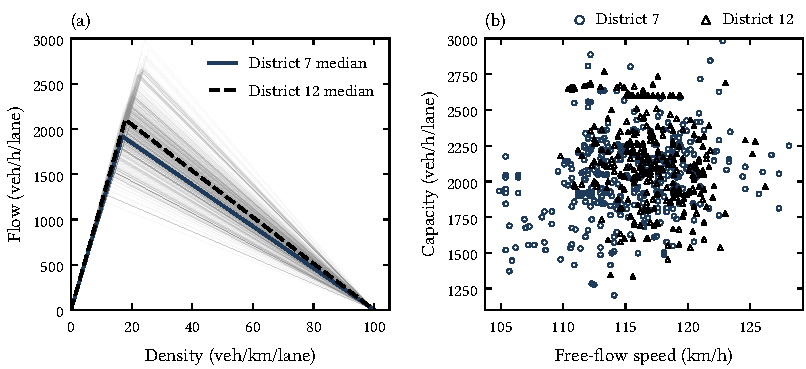
\includegraphics[width=\linewidth]{figures/fig_fundamental_diagram.pdf}
\caption{The physics the evaluator uses. Left: the per-lane triangular diagram of every link (grey) and the
median diagram of each district. Right: free-flow speed against per-lane capacity. Task 3 checks the submitted
speed and flow against these diagrams and against vehicle conservation.}\label{fig:fd}
\end{figure}

\subsection{Masking and eligibility}
A cell is \emph{eligible} when its detector reported for at least 75\,\% of the interval and the required values are
present; about 76\,\% of cells qualify, and only eligible cells are scored in any task. Task 1 removes eligible
cells under three regimes, R1, R2 and R3, at 20, 30 and 50\,\% of cells. Each calendar day belongs to exactly one
regime, so no cell hidden in one view is visible in another. At a blanked cell every measured channel is removed:
speed, flow, occupancy and the occupancy-derived density. The quality flag (\code{pct\_observed}) stays, so the
target cells are known. The Task 2 horizon and the 60 minutes after it are also blanked so that the horizon cannot
be interpolated across.

\subsection{Tasks and scoring}
\paragraph{Task 1, state} For each regime $r$, speed and per-lane flow errors are scored separately and blended,
\begin{equation}
  \begin{aligned}
  \Sstate(r) &= 0.54\,\max\!\Big(0,\,1-\frac{\mathrm{RMSE}_v(r)}{25\ \mathrm{km/h}}\Big)
              + 0.46\,\max\!\Big(0,\,1-\frac{\mathrm{RMSE}_{q/\mathrm{lane}}(r)}{600\ \mathrm{veh/h}}\Big),\\
  \Sstate &= \tfrac13\textstyle\sum_{r\in\{R1,R2,R3\}} \Sstate(r).
  \end{aligned}
  \label{eq:state}
\end{equation}
The equal weight on regimes means the 50\,\% mask counts as much as the 20\,\% mask.

\paragraph{Task 2, queue} A link is \emph{queued} when its latent speed is at most $0.6\,v_f$. Each window provides
the history up to the forecast origin $T$ and asks for the queue field $\hat Y\in\{0,1\}^{L\times 6}$ at
$T{+}5,\dots,T{+}30$ minutes. A window is scored by space-time intersection over union \cite{jaccard1912},
\begin{equation}
  \IoU(\hat Y, Y) = \frac{|\hat Y \wedge Y|}{|\hat Y \vee Y|},
  \label{eq:iou}
\end{equation}
and $\Squeue$ is the mean over windows, five \emph{onset} and five \emph{ongoing} per panel and split. Onset windows
have no queued link anywhere in the history and at least one in the horizon; ongoing windows have a queue at $T$.
Because the two conditions have equal counts, $0.30\,\Squeue = 0.15\,\IoU_{\mathrm{onset}} + 0.15\,\IoU_{\mathrm{ongoing}}$.

\paragraph{Task 3, physics} There are no Task 3 rows. The evaluator forms $k=q/v$ and $N=kL$ from the submitted state
and scores
\begin{equation}
  \Sphys = \tfrac13\,\SFD + \tfrac23\,\SLWR,
  \qquad
  N_{t+\Delta t}-N_t \overset{!}{=} \Delta t\,\big(q_{\mathrm{in}} + q_{\mathrm{on}} - q_{\mathrm{out}} - q_{\mathrm{off}}\big),
  \label{eq:phys}
\end{equation}
where $\SFD$ measures the normalized distance between the submitted flow and the diagram flow at the same density
\cite{lighthill1955,richards1956}, and $\SLWR$ the size of the conservation residual over link-to-link transitions
with the released ramps. All ten corridors use coverage mode A (0.756 ramp coverage).

\paragraph{Task 4, demand} With path-link incidence $A$, released counts $c$ and prior $b$,
$\Sodme = 0.45\,S_{\mathrm{od}} + 0.25\,S_{\mathrm{link}} + 0.15\,S_{\mathrm{dev}} + 0.15\,S_{\mathrm{attr}}$ compares
the submitted path flows $f$ to a withheld reference, $Af$ to $c$, the distance moved from $b$ to the reference's,
and the destination-attraction pattern.

\paragraph{Aggregation} Each component is computed per panel, the two directions of a corridor are averaged, and the
five corridor families are averaged with equal weight. A task with a missing or incomplete row set scores zero.

\subsection{Anatomy of a submission}
A submission has 6,980,503 rows: 6,735,795 \emph{state} rows (speed and flow for every Task 1 target cell of
validation and private), 174,000 \emph{queue} rows (8 panels $\times$ 10 windows $\times$ 1,450 links $\times$ 6
horizons, summed over two splits, half onset and half ongoing) and 70,708 \emph{ODME} rows (35,354 paths $\times$ 2
splits). This arithmetic matters for the analysis in \cref{sec:leaderboard}: the three blocks are disjoint, so each
task's score depends only on its own rows.

\subsection{Five properties of the design that shaped our method}\label{sec:design}
\begin{enumerate}[label=\textbf{P\arabic*.},leftmargin=2.2em]
  \item \textbf{Physics without lookup.} The generator obeys LWR-type physics with calibrated noise, but no external
        record contains the answers. Methods must model the release, not join against outside data.
  \item \textbf{Onsets are placed at the end of the horizon.} The onset selector takes the earliest qualifying
        origin, one whose hour of history has no queue and whose horizon does, with selected origins at least 360
        minutes apart. Simulating that rule on the training split reproduced 39 of the 40 published onset origins. A consequence is that the first queued
        cell almost always appears at $T{+}30$, the last horizon step. The release notes that onsets are visible in
        advance: an hour before a queue forms the road runs at about 1.28 times its queue threshold, against 1.54
        times where none follows, and carries about 6,912 veh/h against 4,620.
  \item \textbf{Ongoing windows are those where persistence fails.} A window is kept only if copying the current
        queue forward scores an IoU of at most 0.9 on it. Trivial persistence is therefore weaker than on random
        congested windows by construction.
  \item \textbf{Queue scores are noisy.} The organizers report a per-window IoU standard deviation of 0.3752 on
        the persistence baseline; with five windows per condition and panel this is about 0.0126 of $\Stotal$ from
        window sampling alone. Validation and private queue scores can differ by that much with no change in skill.
  \item \textbf{Physics cannot be scored locally.} The conservation check needs the organizer's boundary flows,
        which are withheld. Estimating them from the submitted flows swamps the signal: the conservation signal is
        about 0.75\,\% of the vehicles on a link and that estimate is off by about 0.22\,\%, so a perfect answer on
        D12\_I5\_N scores 0.3305 locally and 0.9604 with the organizer flows.
\end{enumerate}

\begin{table}[h]
\centering\small
\caption{Organizer reference scores on the validation split, from the baseline table of the benchmark repository.
These values anchor the additive decomposition of \cref{sec:leaderboard}; our submission of the same baselines
scored 0.55343.}\label{tab:baselines}
\begin{tabular}{@{}l l r r@{}}
\toprule
Component & Naive baseline & Baseline score & Perfect answer \\
\midrule
$\Sstate$ & weekday $\times$ time-of-day historical mean & 0.6929 & 1.0000 \\
$\Squeue$ & persistence of the last history slot & 0.3017 & 1.0000 \\
$\Sphys$ & (inherits the state baseline) & 0.3549 & 0.9636 \\
$\Sodme$ & NNLS against TRAIN counts & 0.8359 & 1.0000 \\
\midrule
$\Stotal$ & & 0.5534 & 0.9945 \\
\bottomrule
\end{tabular}
\end{table}

% ============================================================== PROTOCOL ==
\section{Information boundaries and research protocol}\label{sec:protocol}

\subsection{What each task may read}
Tasks 1, 3 and 4 are offline: the rules allow any released observation of the evaluation split, at any time,
including times after the target cell. Task 2 is online: a forecast for origin $T$ may use released data stamped at
or before $T$. We adopted a stricter contract for Task 2 and kept it in every selected file
(\cref{tab:infosets,fig:t2window}). A forecast reads \emph{exactly} the twelve released slots $T{-}60,\dots,T{-}5$
of its own window, static network data, and models or analogue libraries fitted on the training split. It does not
read slot $T$ (which the current rules allow), other days or windows of the evaluation month, or the offline state
reconstruction. The organizer's own persistence baseline was rewritten to the same twelve slots during the
competition.

\begin{figure}[h]
\centering
\begin{tikzpicture}[x=6.3mm,y=7mm,font=\sffamily\scriptsize]
  % history slots
  \foreach \i in {0,...,11}{
    \fill[accent!78] (\i,0) rectangle ++(0.86,0.86);
  }
  \fill[gridc] (12,0) rectangle ++(0.86,0.86);
  \foreach \i in {13,...,18}{
    \fill[orange!80] (\i,0) rectangle ++(0.86,0.86);
  }
  \foreach \i in {19,...,22}{
    \fill[gridc!70] (\i,0) rectangle ++(0.86,0.86);
  }
  \node[text=white] at (0.43,0.43) {\tiny $-60$};
  \node[text=white] at (11.43,0.43) {\tiny $-5$};
  \node at (12.43,0.43) {\tiny $T$};
  \node[text=white] at (13.43,0.43) {\tiny $+5$};
  \node[text=white] at (18.43,0.43) {\tiny $+30$};
  \draw[decorate,decoration={brace,amplitude=4pt}] (0,1.05) -- (11.86,1.05) node[midway,above=4pt,align=center]
     {\textbf{Read:} 12 released slots, $T{-}60 \dots T{-}5$\\speed, flow, occupancy, ramps, eligibility};
  \draw[decorate,decoration={brace,amplitude=4pt}] (13,1.05) -- (18.86,1.05) node[midway,above=4pt,align=center]
     {\textbf{Predict:} queue field\\$L\times 6$ binary cells};
  \draw[muted,line width=0.4pt] (12.43,-0.12) -- (12.43,-0.42);
  \node[below,align=center,inner sep=1pt] at (12.43,-0.42) {slot $T$: released,\\\emph{not read}};
  \draw[decorate,decoration={brace,amplitude=4pt,mirror}] (19,-0.18) -- (22.86,-0.18) node[midway,below=4pt,align=center]
     {blanked buffer;\\later data never read};
  \node[below,align=center,inner sep=1pt] at (5.43,-0.3)
     {\textbf{+} static network, TRAIN-fitted models,\\TRAIN analogue library};
\end{tikzpicture}
\caption{The Task 2 information contract used in every selected file. Each window reads only its own twelve legal
history slots. Other evaluation days, other windows, slot $T$, ramp values after $T$ and the offline Task 1
reconstruction are excluded.}\label{fig:t2window}
\end{figure}

\begin{table}[h]
\centering\small
\caption{Information sets. ``Allowed'' is the competition rule; ``used'' is what the selected files read.}\label{tab:infosets}
\begin{tabularx}{\linewidth}{@{}l X X@{}}
\toprule
Task & Allowed by the rules & Used by TF3 and ES4 \\
\midrule
1 State & Any released observation of the split, any time; train in full & Masked layer of the same split (target channels absent by construction); TRAIN-fitted trees, profiles, factor and covariance models \\
2 Queue & Released data stamped $\le T$, including earlier days of the split & Exactly $T{-}60\dots T{-}5$ of the window; static network; TRAIN-fitted classifier and TRAIN analogue library \\
3 Physics & No rows; read from Task 1 & --- \\
4 ODME & Split's released counts, prior and incidence & Same; each split solved on its own counts and prior, never TRAIN counts \\
\bottomrule
\end{tabularx}
\end{table}

One early file (\code{P-slotT}, 30 September) set ongoing queues from the state at slot $T$. It was a diagnostic
to measure what slot $T$ adds; it was never a candidate and is not part of either selected file. \Cref{sec:ongoing}
shows that a legal forward-fill of the twelfth slot scores higher than that diagnostic on the public board.

\subsection{A hierarchy of proxies}
Hidden labels exist only on Kaggle, so every decision used one of four local instruments, each with a known weakness.
\begin{enumerate}[label=(\roman*)]
  \item \textbf{Held-out training months.} Models are fitted on June--November and scored on December, January and
        February with the official masks and the official scorers for Tasks 1 and 4. This is the cleanest instrument,
        but training months share one generator draw: they are not new incident schedules.
  \item \textbf{The 80 published training queue windows} (40 onset, 40 ongoing), all dated 1--10 June 2030, scored
        with latent labels reconstructed from the unmasked layer. They are few and repeatedly inspected.
  \item \textbf{Visible-cell pseudo-events in March and April.} Extra masks or pseudo-windows are drawn on cells the
        release shows, with odd and even dates split into development and confirmation halves. The targets are noisy
        observations, not organizer latent labels.
  \item \textbf{A local conservation proxy} that replaces the withheld boundary flux by the observed accumulation
        change. We verified that our implementation equals the official Task 3 scorer given the same flux file, but
        the proxy sits near the exact-answer ceiling and is not the leaderboard physics score.
\end{enumerate}

\subsection{Pre-registered gates}
From 3 October onward each candidate change was registered before its result was seen, with a fixed development
rule, a single confirmation and no rescue. The state ensemble (TS3, \cref{sec:ensemble}) illustrates the template:
\begin{itemize}
  \item \emph{Development} on December and January with models fitted on June--November: the joint proxy
        $0.35\,\Sstate + 0.15\,S_{\mathrm{phys}}^{\mathrm{proxy}}$ must rise by at least 0.0001, $\Sstate$ must not fall,
        at least seven of ten panels must improve and no panel may lose more than 0.001.
  \item \emph{One confirmation} on February with the same rule and at least eight improving panels. A failed arm is
        closed; no member, weight or panel subset is re-selected afterwards.
  \item \emph{Final refit} of the frozen rule on all nine training months, with unchanged seeds and settings.
\end{itemize}
Queue changes used the analogous structure on visible March/April events (odd dates for development, even dates
for confirmation) and on the published June windows, with date-clustered bootstrap intervals.

\subsection{Release engineering}
Every candidate from RC1 (2 October) to TF3 (4 October) passed the checklist below before its single upload.
The later ES files change one column of a frozen, hash-verified parent; each was checked by recomputing its
SHA256 and by a row-level difference against that parent (for example, ES2 changes exactly 1,715,267 speeds and
nothing else). Every file was uploaded once.
\begin{enumerate}
  \item An independent standard-library parser reads all 6,980,503 rows and checks keys, value domains, horizon
        placement and that only the intended columns changed relative to the parent file.
  \item A clean regeneration from the raw release and the saved weights, in a fresh pinned environment that rebuilds
        every cache, must reproduce every queue label exactly and every continuous value to within $10^{-8}$.
  \item The archive SHA256 is recorded and an exclusive attempt marker is created before the single upload call. An
        ambiguous network outcome is never retried; scores are confirmed by a separate read-only listing.
\end{enumerate}

% ========================================================== ARCHITECTURE ==
\section{System architecture}\label{sec:architecture}

\Cref{fig:architecture} shows the deployed pipeline. Three independent lanes produce the three row blocks of the
submission file; Task 3 has no lane of its own and is computed by the evaluator from the state rows. The lanes share
nothing at inference time. In particular, the offline state reconstruction never feeds a queue forecast, which keeps
the Task 2 information set to its twelve history slots. Every learned artefact (trees, profiles, factor and covariance
models, the queue classifier, the onset event pool and the trajectory library) is fitted on the training split,
using the unmasked training layer as labels. The S10 and FS1 flow factors use only the visible cells of the split
being reconstructed.

\begin{figure}[t!]
\centering
% Shared by main.tex (Section 4) and architecture_standalone.tex (README image).
\begin{tikzpicture}[x=1mm,y=1mm,font=\sffamily\scriptsize,
  every node/.append style={execute at begin node={\hyphenpenalty=10000\exhyphenpenalty=10000}},
  stage/.style={draw=#1!65!black,fill=#1!8,rounded corners=2pt,align=center,inner sep=1.6pt,
                text width=24mm,minimum height=11mm,line width=0.45pt},
  lab/.style={draw=none,fill=#1!16,rounded corners=2pt,align=left,inner sep=2.5pt,text width=19mm,
              font=\sffamily\scriptsize,text=#1!55!black},
  arr/.style={-{Stealth[length=3pt,width=2.8pt]},line width=0.55pt,color=ink2},
  darr/.style={-{Stealth[length=3pt,width=2.8pt]},line width=0.55pt,color=ink2,dashed}]

% lane labels
\node[lab=statec,minimum height=26mm] at (11,-7.5) {\textbf{STATE}\\Task 1, offline\\[2pt]masked layer,\\ramps, network};
\node[lab=physc,minimum height=9mm] at (11,-28) {\textbf{PHYSICS}\\Task 3, no rows};
\node[lab=queuec,minimum height=11mm] at (11,-42) {\textbf{ONSET}\\Task 2, 12 slots};
\node[lab=queuec,minimum height=25mm] at (11,-63) {\textbf{ONGOING}\\Task 2, 12 slots\\[2pt]TRAIN classifier\\and library};
\node[lab=odmec,minimum height=11mm] at (11,-85) {\textbf{DEMAND}\\Task 4, own split};

% state
\node[stage=statec] (s1) at (38,0)   {Dense caches\\$[D,288,L]$ grids,\\masked layer};
\node[stage=statec] (s2) at (66,0)   {92 features:\\anchors, ASM,\\neighbours, factors};
\node[stage=statec] (s3) at (94,0)   {3 LightGBM\\members: $v$, $q$\\residuals, density};
\node[stage=statec] (s4) at (122,0)  {Member mean,\\half density\\projection};
\node[stage=statec] (s5) at (38,-15) {S5 free-branch\\speed, rank-8\\covariance};
\node[stage=statec] (s6) at (66,-15) {FS1: S10 factor\\flow, S12 covariance\\speed};
\node[stage=statec] (s7) at (94,-15) {Gap-shell\\link-bias\\recentering};
\node[stage=statec,fill=statec!22,font=\sffamily\scriptsize\bfseries] (s8) at (122,-15) {speed and flow\\per target cell};
\draw[arr] (s1) -- (s2); \draw[arr] (s2) -- (s3); \draw[arr] (s3) -- (s4);
\draw[arr] (s4.south) -- ++(0,-2) -| (s5.north);
\draw[arr] (s5) -- (s6); \draw[arr] (s6) -- (s7); \draw[arr] (s7) -- (s8);

% physics
\node[stage=physc,text width=80mm,minimum height=9mm,dashed] (p1) at (94,-28)
  {Evaluator: \mbox{$k=q/v$} and \mbox{$N=kL$}\\\mbox{$\tfrac13\SFD+\tfrac23\SLWR$} with the released ramps};
\draw[darr] (s8.south) -- (s8.south |- p1.north);

% onset
\node[stage=queuec] (o1) at (38,-42) {13 descriptors\\of the legal hour};
\node[stage=queuec] (o2) at (66,-42) {TRAIN onset events\\within $\pm$30 min,\\same day type};
\node[stage=queuec] (o3) at (94,-42) {10 nearest events,\\standardized\\distance};
\node[stage=queuec,fill=queuec!22] (o4) at (122,-42) {\textbf{Bayes action:}\\max expected IoU,\\mask at $T{+}30$};
\draw[arr] (o1) -- (o2); \draw[arr] (o2) -- (o3); \draw[arr] (o3) -- (o4);

% ongoing
\node[stage=queuec] (g1) at (38,-56) {213 features: lags,\\distance bands,\\characteristics};
\node[stage=queuec] (g2) at (66,-56) {EQ1 classifier\\$p(\ell,h)$, 800 trees,\\3,766 TRAIN windows};
\node[stage=queuec] (g3) at (38,-70) {Encoded history,\\speed and flow\\ratios};
\node[stage=queuec] (g4) at (66,-70) {TRAIN library,\\20 donor\\trajectories};
\node[stage=queuec,minimum height=25mm] (g5) at (94,-63) {Candidate pool\\(up to 34 masks):\\donors, persistence,\\analogue choice,\\decoded $p$, unions,\\mixtures};
\node[stage=queuec,fill=queuec!22,minimum height=25mm] (g6) at (122,-63) {\textbf{RQ48 decoder}\\[3pt]$\arg\max_a$ of\\0.25 empirical IoU\\+ 0.75 model IoU\\[3pt]6 horizons};
\draw[arr] (g1) -- (g2); \draw[arr] (g3) -- (g4);
\draw[arr] (g2.east) -- (g5.west |- g2.east); \draw[arr] (g4.east) -- (g5.west |- g4.east);
\draw[arr] (g5) -- (g6);

% demand
\node[stage=odmec] (d1) at (38,-85) {Incidence $A$,\\counts $c$, prior $b$};
\node[stage=odmec,text width=52mm] (d2) at (80,-85) {$\min_{f\ge0}\ \lVert Af-c\rVert^2+0.05\,\lVert f-b\rVert^2$\\exact NNLS on the stacked system};
\node[stage=odmec,fill=odmec!22,font=\sffamily\scriptsize\bfseries] (d3) at (122,-85) {path flows};
\draw[arr] (d1) -- (d2); \draw[arr] (d2) -- (d3);

% submission
\node[draw=deep,fill=deep,text=white,rounded corners=2.5pt,align=center,text width=17mm,minimum height=96mm,inner sep=2pt]
  (sub) at (151,-42.5) {\textbf{submission}\\\textbf{.csv}\\[2pt]6,980,503\\rows\\[12pt]\textbf{state}\\6,735,795\\[12pt]\textbf{queue}\\174,000\\[12pt]\textbf{odme}\\70,708};
\draw[arr] (s8.east) -- (s8.east -| sub.west);
\draw[arr] (o4.east) -- (o4.east -| sub.west);
\draw[arr] (g6.east) -- (g6.east -| sub.west);
\draw[arr] (d3.east) -- (d3.east -| sub.west);

% training band
\node[draw=rulec,fill=panel2,rounded corners=2pt,align=left,text width=155mm,inner sep=3pt] at (80,-100)
  {\textbf{Fitted on TRAIN only} (June 2030 to February 2031, unmasked layer as labels): state trees and density model,
   weekday $\times$ slot profiles with the own day excluded, rank-8 and rank-24 factor models, S5 and S12 covariances,
   the ongoing classifier, the onset event pool and the trajectory library. S10 and FS1 flow factors use only the
   split's own visible cells.};
\end{tikzpicture}

\caption{Deployed architecture of ES4. TF3 is identical except that it has no gap-shell recentering stage and uses
the earlier Q46 classifier in place of EQ1. Solid arrows denote data flow at inference; the dashed arrow denotes the
evaluator's own computation. No information flows between lanes.}\label{fig:architecture}
\end{figure}

\subsection{Component lineage}
The pipeline grew through single, measured changes. \Cref{tab:lineage} lists each deployed component, the submission
that introduced it and the change in validation score that it produced. \Cref{app:glossary} expands the identifiers.

\begin{table}[h]
\centering\small
\caption{Components of the final submissions. $\Delta$ is the change in validation score of the submission that
introduced the component. Two rows changed two components at once, and the RQ2 value follows from additivity
(CS1 = J1 + RS1 state + RQ2 ongoing, \cref{sec:leaderboard}).}\label{tab:lineage}
\begin{tabularx}{\linewidth}{@{}X l l r c c@{}}
\toprule
Component & Task & Introduced in & $\Delta$ & TF3 & ES4 \\
\midrule
Exact split-specific NNLS demand & ODME & T4-v1 & +0.03158 & \checkmark & \checkmark \\
Residual GBDT on temporal interpolation & State & V1 & +0.12691 & (RS1) & (RS1) \\
Joint-mask onset analogue & Onset & J1 & +0.01861 & \checkmark & \checkmark \\
Forward-filled persistence & Ongoing & U2 & +0.02021 & candidate & candidate \\
RS1 residual model with density reconciliation & State & RC2 & +0.00974 & \checkmark & \checkmark \\
Trajectory-analogue decoder (RQ2) & Ongoing & CS1 & +0.00414 & \checkmark & \checkmark \\
S5 speed correction and Q19 features & State, ongoing & CT1 & +0.00039 & \checkmark & \checkmark \\
S10 factor flow and S12 covariance speed & State & CT2 & +0.00151 & \checkmark & \checkmark \\
FS1 gate and Q46 first-crossing classifier & State, ongoing & CF1 & +0.00449 & \checkmark & FS1 only \\
RQ48 quarter-prior decoder & Ongoing & CF2 & +0.00469 & \checkmark & \checkmark \\
Three-member sample ensemble (TS3) & State & TF3 & +0.00034 & \checkmark & \checkmark \\
All-month ongoing classifier (EQ1) & Ongoing & ES1 & +0.00039 & & \checkmark \\
Gap-shell recentering, shells 1, 2 and 3--6 & State & ES2 to ES4 & +0.00157 & & \checkmark \\
\bottomrule
\end{tabularx}
\end{table}

% ================================================================= STATE ==
\section{Task 1: state reconstruction}\label{sec:state}

\subsection{Formulation}
For one split and panel let $v_{d,t,\ell}$ and $q_{d,t,\ell}$ be speed and flow on day $d$, five-minute slot
$t\in\{0,\dots,287\}$ and link $\ell$ (links in topological order). We store every channel as a dense
$[D,288,L]$ grid. A cell is an \emph{anchor} when it is eligible, finite and not a Task 1 target; target cells
carry no speed, flow or occupancy. For a target cell let $(t^-,t^+)$ be the nearest anchors on the same link and
day, with gaps $g^\pm=|t-t^\pm|$, and let
\begin{equation}
  \tilde v_{d,t,\ell} = \frac{g^+\,v_{d,t^-,\ell} + g^-\,v_{d,t^+,\ell}}{g^-+g^+}
  \label{eq:interp}
\end{equation}
be same-day linear interpolation (edge values are held). Rather than predict $v$ and $q$ directly we predict the
\emph{residuals} $v-\tilde v$ and $q/n_\ell-\tilde q/n_\ell$, where $n_\ell$ is the lane count, so that flow is learned
in the per-lane units of \cref{eq:state}. Interpolation is a strong prior on short gaps; the residual model only
has to learn when and how it is wrong.

\subsection{Baselines}
The organizer baseline predicts a weekday $\times$ time-of-day profile per link and scores $\Sstate=0.6929$ in public.
Same-day interpolation is far stronger, because most gaps are short: of the 3.44 million February training targets,
3.14 million have both anchors within six slots (\cref{fig:state-gaps}). The adaptive smoothing method of
Treiber and Helbing \cite{treiber2002} (ASM) supplies a third estimate. It averages anchors with two exponential
kernels aligned with the free-flow and congested characteristics,
\begin{equation}
  \phi_c(\Delta x,\Delta t) = \exp\!\Big(-\frac{|\Delta x - c\,\Delta t|}{\sigma_x}-\frac{|\Delta t|}{\tau}\Big),
  \qquad c_{\mathrm{free}}=100\ \mathrm{km/h},\ c_{\mathrm{cong}}=-18\ \mathrm{km/h},
  \label{eq:asm}
\end{equation}
with $\sigma_x=0.8$ km and $\tau$ one slot, over $\pm3$ slots and $\pm6$ links, and blends the two estimates with
weight $w=\tfrac12\big(1+\tanh((60-\min(v_{\mathrm{free}},v_{\mathrm{cong}}))/20)\big)$ on the congested one. The
cell itself is excluded, so the estimate at an anchor is leave-one-out.

\subsection{Features}
Every feature is computed from the masked layer, static network files and TRAIN-fitted parameters
(\cref{tab:state-features}). The groups encode four kinds of evidence: the temporal anchors on the same link, the
same-time state of neighbouring links and their own interpolation errors (``innovations''), multiscale and low-rank
summaries of the visible field, and static context. The innovation of a neighbouring anchor,
$\lambda_{t,\ell'} = v_{t,\ell'}-\tilde v^{\,\mathrm{loo}}_{t,\ell'}$, measures how far that link departs from its own
interpolant at the same time, which is direct evidence of a passing wave.

\begin{table}[h]
\centering\small
\caption{The 92 inputs of each state model. ``Neighbour'' means a link $\ell\pm k$ at the same slot. Factor features
are reconstructions from rank-8 and rank-24 temporal factor models fitted on TRAIN.}\label{tab:state-features}
\begin{tabularx}{\linewidth}{@{}l X r@{}}
\toprule
Group & Features & Count \\
\midrule
Temporal anchors & interpolated $v$, $q$; previous and next anchor values and gaps; previous occupancy & 9 \\
Adaptive smoothing & ASM speed and flow, free-flow and congested kernel estimates & 4 \\
Profiles and ramps & weekday $\times$ slot TRAIN profile of $v$ and $q$ (own day excluded); on- and off-ramp flow & 4 \\
Neighbour state & $v$, $q$ and their innovations at $\ell\pm1,\pm2,\pm3$; innovations of $\ell\pm1$ one slot before and after & 28 \\
Static and calendar & lanes, free-flow speed, capacity, length, position; slot, weekday, regime, observation rate; panel & 11 \\
Multiscale speed & interpolation, gap, rank-8 and rank-24 factor fit, four box smooths ($1$ or $3$ slots $\times$ 7 or 21 links), near links $\pm1,\pm2$ & 12 \\
Multiscale flow & the same twelve for per-lane flow & 12 \\
Multiscale occupancy & interpolation, four box smooths, near links $\pm1,\pm2$ & 9 \\
Density and quality & interpolated $q/v$, $\tilde q/\tilde v$; \code{pct\_observed} of the target cell & 3 \\
\midrule
Total & & 92 \\
\bottomrule
\end{tabularx}
\end{table}

\subsection{Learner}
Three LightGBM \cite{ke2017} regressors are trained per member on pooled panels with the panel as a categorical
feature: the speed residual and the per-lane flow residual under squared error, and density $k$ under absolute
error. Settings are fixed and were never tuned on evaluation months (\cref{tab:hyper}). The final fit samples up to
600,000 eligible target cells per panel, six million in total, from the 31,783,763 eligible TRAIN target cells.

\begin{table}[h]
\centering\small
\caption{State-model settings, identical for every member. There is no early stopping.}\label{tab:hyper}
\begin{tabular}{@{}l r l r@{}}
\toprule
Setting & Value & Setting & Value \\
\midrule
Boosting rounds & 800 & Feature fraction & 0.9 \\
Leaves & 255 & Bagging fraction (every round) & 0.8 \\
Learning rate & 0.05 & $L_2$ penalty & 2 \\
Minimum leaf size & 150 & Rows per panel and member & $\le$ 600,000 \\
Objectives & \multicolumn{3}{l}{squared error for $v$ and $q$ residuals; absolute error for density} \\
\bottomrule
\end{tabular}
\end{table}

\paragraph{Density reconciliation} The three predictions $(\hat v,\hat q,\hat k)$ need not satisfy $q=kv$. We take a
half step of the first-order, error-weighted projection onto that constraint. With $a=-\hat q/\hat v^2$, $b=1/\hat v$,
$r=\mathrm{clip}(\hat k-\hat q/\hat v,-10,10)$, $\sigma_v=1.5$ km/h, $\sigma_q=30$ veh/h/lane and
$D=a^2\sigma_v^2+b^2\sigma_q^2$,
\begin{equation}
  v \leftarrow \mathrm{clip}\Big(\hat v + \tfrac12\,\frac{r\,a\,\sigma_v^2}{D},\,5,\,140\Big),\qquad
  q \leftarrow \max\Big(0,\ \hat q + \tfrac12\,\frac{r\,b\,\sigma_q^2}{D}\Big).
  \label{eq:density}
\end{equation}
The scales distribute the correction in proportion to each channel's typical error, so a density disagreement
moves flow more than speed.

\subsection{Free-branch corrections}\label{sec:freebranch}
On the free-flow branch the residual model's errors are small but spatially correlated. Three statistical
corrections act only there; none enforces the diagram or conservation exactly.
\begin{itemize}
  \item \textbf{S5, speed.} A rank-8 spatial covariance of free-flow speeds, fitted on June--November TRAIN, conditions
        each masked link on the same-time observed links. It applies where $\hat v>0.92\,v_f$, $\hat q<0.8$ capacity and
        the link had at least 100 free-flow observations.
  \item \textbf{S10, flow.} A rank-12 factor model of transformed per-lane flow and occupancy is fitted to one evaluation
        month's \emph{visible} free-flow cells, with link-wise centering, channel scaling, and diagonal autoregressive
        penalties at lags 1--3 on the temporal factors that never cross a day boundary (24 alternating ridge updates).
        The temporal penalty follows temporal regularized matrix factorization \cite{yu2016}. This is legal offline
        adaptation: target channels are absent, and no label is read.
  \item \textbf{S12, speed.} A full spatial covariance of June--November TRAIN free speeds, projected to positive
        definite form with 5\,\% diagonal shrinkage, gives the conditional mean of the missing links $M$ given the
        observed links $O$ at the same time,
        \begin{equation}
          v^{\mathrm{cond}}_M = \mu_M - P_{MM}^{-1}P_{MO}\,\big(v_O-\mu_O\big),\qquad P=\Sigma^{-1}.
          \label{eq:s12}
        \end{equation}
\end{itemize}
The deployed gate FS1 widens the region to $v_0>0.85\,v_f$ and $q_0<0.9$ capacity, evaluated on the S5 output
$(v_0,q_0)$, and blends at half strength: $q=\tfrac12 q_0+\tfrac12 q^{\mathrm{factor}}$ and
$v=\mathrm{clip}(\tfrac12 v_0+\tfrac12 v^{\mathrm{cond}},5,140)$. On February the fixed half-strength arm beat its
predecessor on every panel (joint proxy gain +0.000156). The public board measured S10/S12 at +0.00151 (CT2 against CT1,
state only); FS1 shipped together with a queue change.

\subsection{A fixed three-member sample ensemble}\label{sec:ensemble}
A single tree ensemble fitted on one random sample of six million cells gives a slightly different field than a
fit on another sample. For member predictions $p_m$, their mean $\bar p$ and any target $y$,
\begin{equation}
  \frac1M\sum_{m=1}^M (p_m-y)^2 - (\bar p-y)^2 = \frac1M\sum_{m=1}^M (p_m-\bar p)^2 \;\ge\; 0,
  \label{eq:ambiguity}
\end{equation}
so averaging improves on the mean member by exactly the members' spread \cite{breiman1996}. TS3 averages three
members: the frozen RS1 regressors and two refits with seeds 20261104 and 20261204, each drawing up to 600,000
eligible rows per panel without replacement. The raw speed and flow predictions are averaged with equal weight
and \cref{eq:density} and the free-branch corrections are applied once, to the average. No member was dropped and
no weight tuned after a score was seen.

The protocol of \cref{sec:protocol} was registered before fitting. \Cref{tab:ts3} shows the development and
confirmation results against a control that reproduced the parent exactly; the rule was then refit on all nine
months and shipped as TF3, which measured +0.00034 in public.

\begin{table}[h]
\centering\small
\caption{TS3 against its exact parent on held-out TRAIN months (models fitted on June--November). All ten panels
improved in every month. TRAIN proxies, not leaderboard scores.}\label{tab:ts3}
\begin{tabular}{@{}l r r r r@{}}
\toprule
Month (role) & $\Delta\Sstate$ & $\Delta S_{\mathrm{phys}}^{\mathrm{proxy}}$ & $\Delta(0.35\,\Sstate+0.15\,S_{\mathrm{phys}}^{\mathrm{proxy}})$ & Panels improved \\
\midrule
December (development) & +0.00032340 & +0.00172636 & +0.00037214 & 10 / 10 \\
January (development)  & +0.00033570 & +0.00178485 & +0.00038522 & 10 / 10 \\
February (confirmation) & +0.00025537 & +0.00152578 & +0.00031825 & 10 / 10 \\
\bottomrule
\end{tabular}
\end{table}

\subsection{Short-gap link-bias recentering}\label{sec:recenter}
\paragraph{Observation} On February training targets, the same-day interpolant \cref{eq:interp} is almost unbiased
\emph{per link} when both anchors are close: the mean absolute per-link bias of $\tilde v-v$ is about 0.02 km/h on
one-slot gaps. The deployed reconstruction is not. On March, ES1's per-link means sit 0.77--1.54 km/h (RMS across
links, by panel) from the same interpolant on one-slot cells. A model fitted on June--February carries a month-level
offset into a new month; the interpolant, built from that month's own anchors, does not.

\paragraph{Estimator} The \emph{gap shell} $G_{[a,b]}$ is the set of target cells that have both anchors and satisfy
$a\le\max(g^-,g^+)\le b$. Because the interpolant's link bias on a passing shell is negligible,
\begin{equation}
  \mathbb E\big[\hat v-v \,\big|\, \ell, G\big] \;\approx\; \mathbb E\big[\hat v-\tilde v \,\big|\, \ell, G\big]
  \;=\; \delta_\ell ,
  \label{eq:recenter}
\end{equation}
and the right-hand side needs no label. For each split, panel and link with at least 100 shell cells we compute
$\delta_\ell$ as the mean of $\hat v-\tilde v$ over the shell and set $v\leftarrow\mathrm{clip}(\hat v-\delta_\ell,5,140)$.
This removes the link-mean component of the error, $\mathrm{MSE}=\mathrm{bias}^2+\mathrm{variance}$, and keeps
the model's within-link structure; it never replaces the model by the interpolant, which loses on hard cells
(\cref{sec:state-error}).

\paragraph{Gates} A shell passes on February when the interpolant's mean absolute link bias is below 0.15 km/h and a
bias correction estimated on earlier months does not raise February RMSE by more than 0.02 km/h. A passing shell is
written to a panel and split only if the RMS link shift is at least 0.40 km/h and no link moves by more than 15 km/h.
Flow was not recentered: its February link bias (3--10 veh/h) is negligible against an RMSE near 200 veh/h, and the
March link offset of the flow interpolant (10.9 veh/h RMS) missed its 20 veh/h bar.

\begin{figure}[t]
\centering
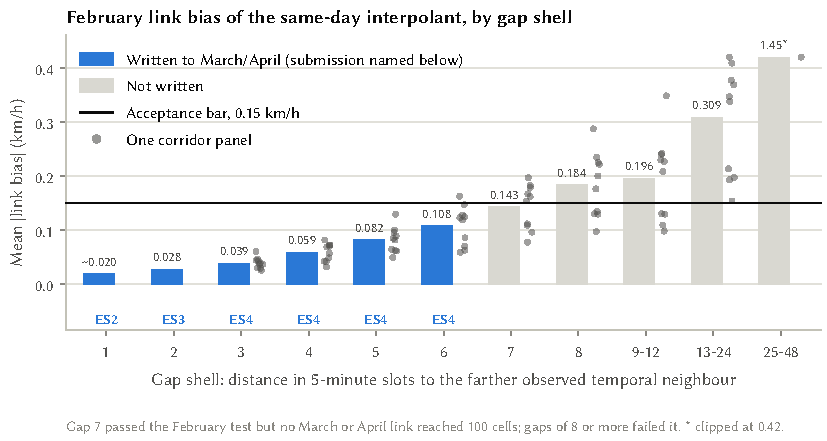
\includegraphics[width=\linewidth]{figures/fig_gap_ladder.pdf}
\caption{The bias test that decided which shells were written. Bars: February mean absolute link bias of the
same-day interpolant, pooled over panels; dots: individual panels. Shells 1--6 passed and were written in three
submissions. Shell 7 passed but no March or April link had the 100 cells the writing rule requires.}\label{fig:gap-ladder}
\end{figure}

\begin{table}[h]
\centering\small
\caption{The gap-shell ladder. February columns are TRAIN proxies; ``changed'' counts March and April speeds;
public $\Delta$ is the Kaggle change of the submission that wrote the shell.}\label{tab:ladder}
\begin{tabular}{@{}l r r r r l@{}}
\toprule
Shell (slots) & Feb.\ link bias & Feb.\ RMSE raw $\rightarrow$ corrected & Speeds changed & Mean $|\Delta v|$ & Public $\Delta$ \\
\midrule
1        & $\approx$0.02 & unchanged & 1,715,267 & 0.962 & +0.00039 (ES2) \\
2        & 0.028 & 2.560 $\rightarrow$ 2.560 & 1,918,477 & 0.960 & +0.00044 (ES3) \\
3        & 0.039 & 2.842 $\rightarrow$ 2.842 & 1,186,051 & \multirow{4}{*}{0.954} & \multirow{4}{*}{+0.00074 (ES4)} \\
4        & 0.059 & 3.085 $\rightarrow$ 3.086 & 671,422 & & \\
5        & 0.082 & 3.423 $\rightarrow$ 3.425 & 319,161 & & \\
6        & 0.108 & 3.562 $\rightarrow$ 3.565 & 15,289 & & \\
7        & 0.143 & 3.646 $\rightarrow$ 3.651 & 0 & --- & not written \\
8        & 0.184 & --- & 0 & --- & failed \\
9--12    & 0.196 & --- & 0 & --- & failed \\
13--24   & 0.309 & --- & 0 & --- & failed \\
25--48   & 1.451 & --- & 0 & --- & failed \\
\bottomrule
\end{tabular}
\end{table}

Across the three submissions the edit changed 5,825,667 speeds by about 0.96 km/h on average (RMS 1.25 km/h,
maximum 6.24 km/h) and added +0.00157 in public. It is a small gain from a simple, label-free statistic, and it is
the only evaluation-month adaptation of speed in the selected files.

\subsection{Results and error analysis}\label{sec:state-error}
\Cref{fig:state-regimes} compares the RS1 residual model with interpolation on February, held out from a fit on
June--November. Speed RMSE falls from 2.75--2.98 to 1.46--1.66 km/h and per-lane flow RMSE from 44.5--47.6 to
30.4--31.1 veh/h, giving a state piece of 0.940--0.945 against 0.899--0.907. The 50\,\% mask costs the model only
0.005 in the piece relative to the 20\,\% mask. \Cref{fig:state-gaps} shows that the advantage holds at every gap
length: the model roughly halves interpolation error from one-slot gaps (1.41 against 2.37 km/h) to gaps of 13--30
slots (1.99 against 3.98 km/h).

\begin{figure}[t]
\centering
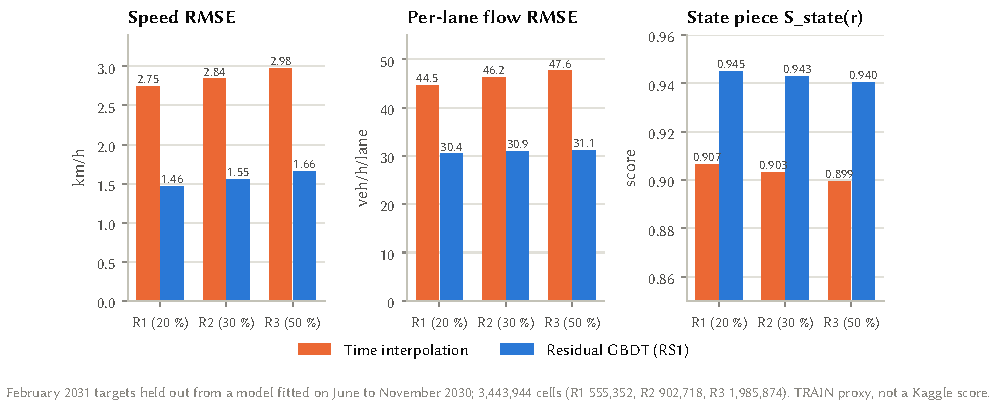
\includegraphics[width=\linewidth]{figures/fig_state_regimes.pdf}
\caption{February state error by masking regime for the residual model and for same-day interpolation.}\label{fig:state-regimes}
\end{figure}

\begin{figure}[t]
\centering
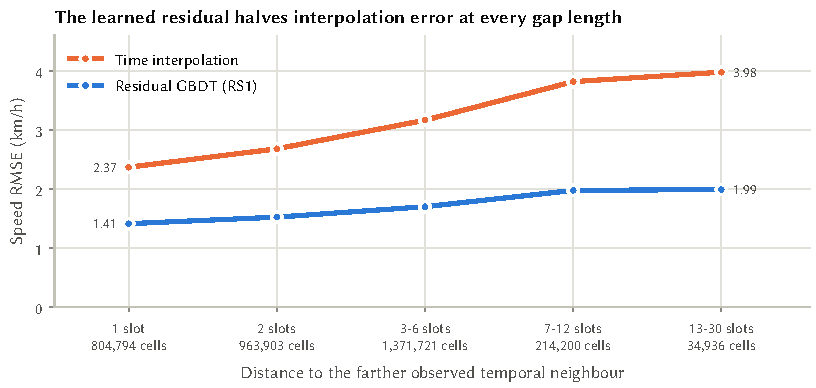
\includegraphics[width=\linewidth]{figures/fig_state_gaps.pdf}
\caption{February speed error by gap length. The residual model's error grows from 1.41 to 1.99 km/h as gaps widen;
interpolation's grows from 2.37 to 3.98 km/h.}\label{fig:state-gaps}
\end{figure}

\paragraph{Where the error is} Error concentrates where a wave passes inside the gap. Among February cells with both
anchors within six slots, 138,195 have anchors that disagree by at least 20 km/h or an interpolant at most
$0.6\,v_f$. There interpolation reaches
10.57 km/h RMSE and the model 4.62 km/h, better on all ten corridors. Same-time neighbours do not substitute for
temporal anchors: on 735,668 cells where both adjacent links are observed, their average scores 6.37 km/h against the
model's 1.44, and switching to the neighbours only when the temporal anchors disagree by 20 km/h still scores
1.60 km/h. The model already combines both sources better than any fixed rule we tried.

\paragraph{What the public board says} Replacing the first residual model by plain interpolation (L0 against U2)
cost 0.00867 in public, and the RS1 model added +0.00974 over the first model (RC2 against RC1). Month-blocked
cross-validation on training months had predicted about +0.021 for the first model over interpolation in the same
state-and-physics block, $0.35\,\Sstate+0.15\,\Sphys$; the public board measured +0.0087. The model transfers to a new month, but less than half
of its cross-validated advantage survived, which is why every later state change was gated on held-out months
and why we treat state proxies as optimistic by a factor of about two.

% =============================================================== PHYSICS ==
\section{Task 3: physics consistency}\label{sec:physics}

Task 3 has no rows. Its 15\,\% weight is earned or lost by the Task 1 answer, through the two terms of
\cref{eq:phys}. This section explains why we ended up \emph{not} imposing physics on the reconstruction, after
testing it many ways.

\subsection{The diagram term is saturated}
$\SFD$ compares the submitted per-lane flow with the triangular diagram at the submitted density. Any field whose
speed and flow are jointly plausible satisfies it. Scored against the released \code{fd\_parameters.csv}, ES4's own
speed and flow reach 0.984--0.994 on all twenty panel-splits of validation and private, with a mean absolute flow
residual of 5--15 veh/h and essentially no clipping. Exact observations score about 0.986 on the training months. A
projection of the field onto the diagram buys about +0.002 in $\Sphys$ and costs speed accuracy, so it was not used.

\subsection{The conservation term cannot be measured locally}
$\SLWR$ checks $N_{t+\Delta t}-N_t$ against boundary flows that the organizers compute from their own state. Those flows
are withheld. Our local scorer is a line-by-line equivalent of the official one: given the same boundary-flux file,
the two agree to four decimal places on eight test fields and four panels. With the flux replaced by the observed accumulation
change, it sits near the exact-answer ceiling (the organizers' perfect answer scores 0.9636 in $\Sphys$, about 0.95 in
$\SLWR$), so it is optimistic and compresses differences between methods. We therefore used it only as a
non-regression check next to $\Sstate$, never as the objective.

\subsection{Imposing physics lost every time}
We tested the most natural ways to make the reconstruction obey the kinematic-wave model \cite{lighthill1955,richards1956,treiber2013}.
Each was frozen on fitting months and scored once on held-out months (\cref{fig:physics,tab:physics}).

\begin{figure}[t]
\centering
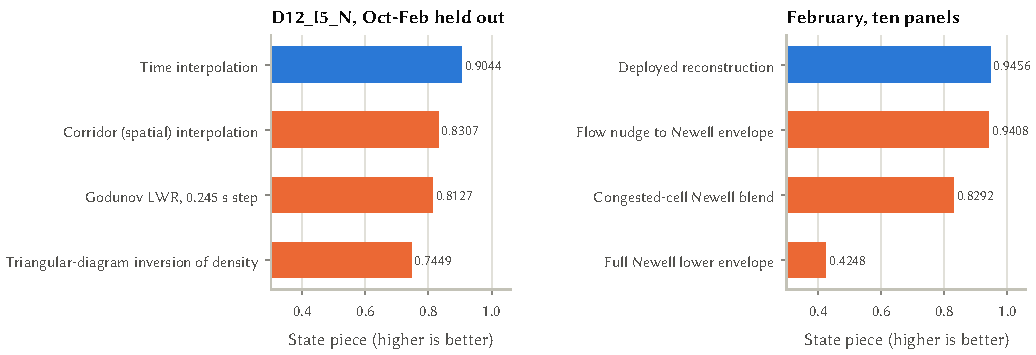
\includegraphics[width=\linewidth]{figures/fig_physics_alternatives.pdf}
\caption{Physics-based reconstructions against their controls. Left: one corridor, all October--February targets
(2,583,593 cells), where same-day interpolation is the control. Right: February on all ten panels, where the
deployed residual model is the control. Blue marks the control; TRAIN proxies.}\label{fig:physics}
\end{figure}

\begin{table}[h]
\centering\small
\caption{Physics-based reconstruction experiments. ``Piece'' is the per-cell state score of \cref{eq:state}. All
numbers are held-out TRAIN proxies; none of these variants is in a selected file.}\label{tab:physics}
\begin{tabularx}{\linewidth}{@{}X r r X@{}}
\toprule
Method & Piece & Control & Outcome \\
\midrule
Godunov LWR, 0.245 s step, 1,224 substeps per bin, released diagram, visible cells pinned \cite{godunov1959,daganzo1994} & 0.8127 & 0.9045 & congested speed RMSE 20.68 vs 8.10 km/h; gate +0.005 failed \\
Corridor (spatial) interpolation of speed and flow & 0.8307 & 0.9045 & speed RMSE 6.59 vs 2.93 km/h \\
Diagram inversion of spatially interpolated density & 0.7449 & 0.9045 & flow RMSE 104.3 vs 42.1 veh/h/lane \\
Steady flux $\min(\text{sending},\text{receiving})$ on 1,159,377 ramp-free holes & 0.8510 & 0.9074 & congested speed RMSE 18.60 vs 7.98 km/h \\
Time-interpolated speed with corridor-interpolated flow & $+$0.0037 & --- & lost on two corridors; local physics lower on seven \\
Newell lower envelope of cumulative counts \cite{newell1993} & 0.4248 & 0.9456 & speed RMSE 79.03 vs 1.60 km/h \\
Newell envelope only on congested cells & 0.8292 & 0.9456 & speed RMSE 7.36 km/h \\
Flow nudge of at most 40 veh/h/lane toward the envelope & 0.9408 & 0.9456 & physics proxy 0.700 vs 0.743; projected $-$0.0081 total \\
Congested-branch diagram flow from the interpolated speed & --- & --- & 101.4 vs 63.3 veh/h/lane on 131,696 cells, worse on all ten panels \\
Occupancy density $k=285\cdot\mathrm{occ}$ inverted through the diagram & --- & --- & below interpolation on all ten panels \\
Flow--ramp balance regression on consecutive visible pairs & --- & --- & held-out correlation 0.0009--0.0094 (bar 0.5) \\
\bottomrule
\end{tabularx}
\end{table}

\subsection{Why physics loses here}
The results share one explanation. The masked holes are short in space and time. On D12\_I5\_N, of 1,159,377
ramp-free target cells with a detector on both sides, 494,175 sit in one-link holes, 345,813 in two-link holes and
295,706 in holes of three to five links; no hole is longer than twenty links. The information about a missing cell
is mostly in its own detector a few minutes earlier and later. A fine-step solver moves a wave across the whole hole
within one five-minute bin, so its five-minute aggregate becomes a \emph{spatial} reconstruction, and spatial
reconstruction is the weaker estimator (corridor interpolation 0.831 against temporal 0.904; the solver scores 0.813).
Beyond that, incidents and capacity drops in the generator are unobserved forcing; a detector's five-minute flow is
not the cell-boundary flux of the conservation check; and the conservation signal itself is small (about 0.75\,\% of
the vehicles on a link) relative to the measurement noise.

\begin{keybox}[Insight]
In this benchmark the physics weight is best served by an accurate state, not by a physical model of the state.
The diagram term is satisfied by any accurate field, and the conservation term moved together with state accuracy in
every held-out test (for example, TS3 raised the local physics proxy by +0.0015 to +0.0018 while raising $\Sstate$).
Imposing the kinematic-wave model never beat temporal evidence on held-out months.
\end{keybox}

% ================================================================= QUEUE ==
\section{Task 2: queue forecasting}\label{sec:queue}

\subsection{Formulation}
A window $w$ has origin $T$ and history $H_w$: speed, flow, occupancy, eligibility and ramp counts on the twelve slots
$T{-}60,\dots,T{-}5$ (\cref{fig:t2window}). We must output a binary field $a\in\{0,1\}^{6\times L}$ over links and the
six horizons. The decision that maximizes the expected score is
\begin{equation}
  a^\star(H_w) = \arg\max_{a}\ \mathbb E\big[\IoU(a,Y)\,\big|\,H_w\big],
  \label{eq:bayes}
\end{equation}
which has no closed form because IoU is a ratio over the whole field \cite{nowozin2014}. We approximate the
expectation in two ways. An \emph{empirical} estimate averages the IoU of $a$ against the complete outcomes $y_j$ of
analogous training windows \cite{lorenz1969}. A \emph{model} estimate uses per-cell probabilities $p_i$ and the ratio of
expected intersection to expected union,
\begin{equation}
  \widehat{\IoU}_p(a) = \frac{\sum_i a_i p_i}{\sum_i a_i + \sum_i p_i - \sum_i a_i p_i}.
  \label{eq:modeliou}
\end{equation}
This ratio of expectations is not the exact expected IoU, but it rewards the right trade-off between size and
confidence, which a per-cell threshold does not.

\subsection{What the window selection implies}
Two properties of the selector (\cref{sec:design}) decide the shape of a good forecaster.
\begin{itemize}
  \item \textbf{Onset queues appear at the last step.} In the 40 published training onset windows the median first
        crossing of $0.6\,v_f$ is at horizon 6. The head of the queue is usually a recurrent bottleneck whose location
        a training prior already contains: the top three links of a frequency prior include it in 79\,\% of events. The
        size is the hard part. With a perfect head and an unknown extent a contiguous block scores about 0.62 latent IoU;
        with the true extent, 0.905. Extent varies from one to eight links and we found nothing in the legal hour that
        predicts it (correlation 0.05 with daily demand, 0.10 with hourly demand).
  \item \textbf{Ongoing windows are those persistence gets wrong.} Windows with persistence IoU above 0.9 are excluded.
        In 31 of the 40 published ongoing windows the queue began before $T{-}60$, so most queues are mature, and their
        evolution over the next 30 minutes (clear, hold or grow) is the forecast.
\end{itemize}

\subsection{Ongoing queues: start by not dropping sensors}\label{sec:ongoing}
The organizer's persistence baseline repeats the queue state of slot $T{-}5$ using eligible cells only. Between 23 and
24\,\% of links have a missing or ineligible $T{-}5$ reading in every split, and persistence then predicts ``not
queued'' there. Forward-filling the last \emph{released} value of each link over the twelve slots, ineligible readings
included, keeps those links. On the public board this raised ongoing IoU from about 0.603 to 0.738 (U2 against U1,
an ongoing-only change of +0.02021 in total). A diagnostic that set ongoing queues from the state at slot $T$
(P-slotT) reached only about 0.729. On the training windows slot $T$ adds $+0.003\pm0.002$ latent IoU over the legal
forward-fill: what mattered was not the extra slot but not throwing away the sensors that were already there.

\subsection{Onset: a joint-mask analogue}\label{sec:onset}
Per-link classifiers decide each link independently and so cannot represent the joint size and shape of an onset.
The J1 rule instead chooses a complete mask from the outcomes of similar training events.
\begin{enumerate}
  \item \textbf{Event pool.} Training origins that meet the legal onset definition (no queue in $T{-}60\dots T{+}25$,
        a queue at $T{+}30$, history coverage at least 0.7), within $\pm30$ minutes of the query origin. Candidates are
        tiered: same day type (weekday or weekend) and local time first, then any day type, then any slot.
  \item \textbf{Similarity.} Thirteen descriptors of the legal hour: total flow over capacity (last, mean, change), the
        mean speed-to-threshold ratio (last, mean, change), the minimum ratio, the eligibility rate, total ramp flow
        (last, mean, change), and the sine and cosine of the time of day. Distance is the standardized RMS difference,
        and the ten nearest events are kept.
  \item \textbf{Action set.} Each neighbour's observed $T{+}30$ mask, plus the top-$k$ links of the neighbours' marginal
        frequency for $k=1,\dots,15$.
  \item \textbf{Bayes action.} The action with the highest mean IoU against the ten neighbour outcomes on their known
        cells, placed at $T{+}30$ only; horizons 1--5 are empty.
\end{enumerate}
In public, the legal LightGBM onset classifier scored about 0.626 IoU, a frequency prior 0.450 and J1 0.750
(\cref{tab:components}). J1 has been the onset of every candidate since, including both selected files. Its 0.75 is
close to what the training analysis says twelve slots allow (0.62 with unknown extent, 0.905 with the true extent).

\subsection{Ongoing queues: classifier, analogue library and decoder}\label{sec:decoder}
\paragraph{Training population} A training origin is \emph{difficult} when its observed six-step future has queued
cells, its denoised origin state has a queue, and six-step persistence scores at most 0.9 IoU on it, mirroring the
selector. A \emph{first crossing} is a difficult origin whose predecessor was not difficult. Q46 was fitted on 2,093
first crossings from July--November (at most 300 per panel). EQ1, in ES4, keeps every one of them and adds up to 240
date-diverse first crossings per panel from June, December, January and February: 3,766 windows and 3,172,453 rows.
Future training observations are labels only, never inputs.

\paragraph{Features} 213 inputs per link and horizon, all from the twelve legal slots (\cref{tab:queue-features}).
Beyond lags and summaries, two groups carry the traffic physics. Distance bands summarize the speed ratio, flow ratio
and density 1, 2, 4, 8 and 16 km upstream and downstream. Characteristic features read the state along the free-flow
and backward-wave characteristics through each link, at ages of 0, 15 and 30 minutes, which is where a wave that will
reach the link within the horizon is visible now.

\begin{table}[h]
\centering\small
\caption{The 213 inputs of the ongoing-queue classifier.}\label{tab:queue-features}
\begin{tabularx}{\linewidth}{@{}l X r@{}}
\toprule
Group & Features & Count \\
\midrule
Lags & speed and flow at lags 1, 2, 3, 4, 6, 9, 12 slots & 14 \\
Summaries & recent, previous, early, min, max, std, slope, trend, coverage, age; for speed and flow & 20 \\
Neighbours & last value and trend at links $\pm1,\pm2,\pm4$; for speed and flow & 24 \\
Corridor & corridor mean, minimum and trend; for speed and flow & 6 \\
Queue context & queued neighbours at $\pm1,\pm2,\pm3$, queued count and its change, nearest queue up- and downstream & 10 \\
Density & $q/v$ density, last value, trend, acceleration, distance to the queue cut & 5 \\
Distance bands & speed ratio, flow ratio and density at $\pm1,2,4,8,16$ km: recent, trend, extreme & 90 \\
Characteristics & free-flow and wave characteristics, both directions, ages 0/3/6 slots; speed, flow, density & 36 \\
Static and calendar & free-flow speed, per-lane capacity, lanes, length, per-lane jam density; slot, weekend, horizon & 8 \\
\midrule
Total & & 213 \\
\bottomrule
\end{tabularx}
\end{table}

\paragraph{Classifier} A LightGBM binary model with 63 leaves and learning rate 0.05, equal weight per panel and per
window, and the horizon as an input, so one model covers all six steps. Q46 has 400 trees; EQ1 has 800.

\paragraph{Analogue library} Every training origin, at a stride of two slots, is encoded by its twelve-slot speed and
flow ratios and its complete six-step future. For a query, donors are restricted to $\pm2$ hours of time of day and the
same weekend flag when at least 20 such donors exist. The distance is the mean squared difference of the speed-ratio
history, with links currently below $0.85\,v_f$ weighted thirteen times, plus 0.4 times the flow-ratio distance, plus
0.15 times one minus the Jaccard overlap of the current queue sets. The 20 nearest donors are kept.

\paragraph{Candidate pool} The decoder chooses among at most 34 complete masks: the analogue's own choice; persistence;
the expected-count decoding of $p$; $p\ge0.4$ and $p\ge0.5$; the 20 donor futures; the donors' marginal frequency
thresholded at 0.25, 0.40, 0.55 and 0.70; the union and intersection of the analogue choice with the decoded $p$; and
the expected-count decoding of $\alpha\,\text{marginal}+(1-\alpha)\,p$ for $\alpha\in\{0.25,0.5,0.75\}$.

\paragraph{Decoder (RQ48)} With $\widehat{\IoU}_{\mathrm{emp}}(a)$ the mean IoU of $a$ against the donor futures on their
known cells, the deployed choice is
\begin{equation}
  \hat a = \arg\max_{a\in\mathcal A}\ \Big[\,0.25\,\widehat{\IoU}_{\mathrm{emp}}(a) + 0.75\,\widehat{\IoU}_p(a)\,\Big].
  \label{eq:rq48}
\end{equation}
The earlier rule used equal weights. Four weightings were registered before development; the quarter weight had
the largest minimum gain across the March and April development samples, passed its single confirmation
(+0.0335 and +0.0300 on even dates, date-clustered 95\,\% intervals [0.013, 0.054] and [0.012, 0.051]), and measured
+0.00469 in public, which corresponds to +0.031 ongoing IoU.

\subsection{Results and the selection gap}\label{sec:queue-results}
\Cref{tab:components} gives the public evidence. Ongoing IoU rose from about 0.603 (organizer persistence) to 0.738
(forward-fill) and 0.766 (first analogue decoder); two later steps changed the state as well and cannot be split, then
RQ48 added +0.031 and EQ1 +0.003. If the two state corrections in those mixed steps contributed between nothing and
their full held-out proxy value, ES4's ongoing IoU is between 0.827 and 0.832 in public. Onset stayed at 0.750.

\begin{figure}[t]
\centering
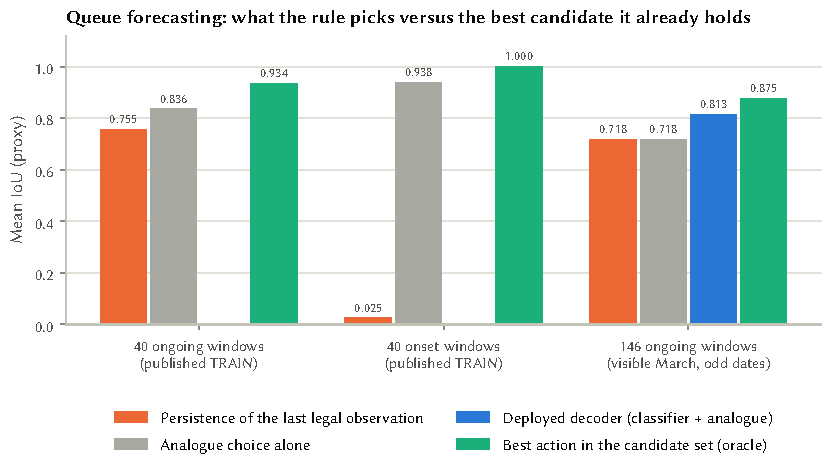
\includegraphics[width=\linewidth]{figures/fig_queue_ceiling.pdf}
\caption{The selection gap. ``Best action'' is the highest-scoring mask already in the candidate set, identified with
the label after the choice; it is a diagnostic, not a forecast. Published windows use latent labels; March windows
use visible observations. The full decoder was not scored on the June instrument.}\label{fig:queue-ceiling}
\end{figure}

\Cref{fig:queue-ceiling} shows where the remaining queue error lives. On the 40 published ongoing windows, the
analogue's choice scores 0.836 while the best mask in its own candidate set scores 0.934. On 146 visible March
windows the deployed decoder scores 0.813 against a best-in-set 0.875, and the analogue's choice alone ties
persistence (0.718). On 160 hard November windows the best whole-window action scores 0.946 and the best per-link
combination 0.967, against 0.807 for the deployed whole-window rule. The candidates are good enough; choosing among
them is not. None of the frozen selection rules we tried cleared its pre-set gain on held-out windows (0.02--0.03
IoU): a ridge reranker (+0.007), an expected-overlap-minus-disagreement ranker (+0.009), a cell majority of the 20
donors (+0.004), a neighbour-bit classifier ($-0.010$), per-link nearest-neighbour copies ($-0.022$), odd-date panel
weights and a March-fit reranker (\cref{sec:negative}).

\begin{keybox}[Insight]
Queue forecasting here is a decision problem over complete masks. The two largest gains came from keeping
information (forward-filling dropped sensors) and from respecting the joint structure of the outcome (choosing whole
onset masks by expected IoU). Better per-cell probabilities moved the score less than the choice among whole masks,
and that choice, not the candidate set, is where the remaining error sits.
\end{keybox}

% ================================================================== ODME ==
\section{Task 4: path-flow and OD estimation}\label{sec:odme}

\subsection{Formulation}
Each panel ships a path set (one path per upstream-to-downstream zone pair, \cref{tab:corridors}), the path-link
incidence $A\in\{0,1\}^{|\mathcal L|\times|\mathcal P|}$, the split's link counts $c$ and a weak path-flow prior $b$.
We solve, separately for validation and for private,
\begin{equation}
  f^\star = \arg\min_{f\ge 0}\ \lVert Af-c\rVert_2^2 + \lambda\,\lVert f-b\rVert_2^2,\qquad \lambda=0.05,
  \label{eq:odme}
\end{equation}
a generalized least-squares estimator in the tradition of Cascetta \cite{cascetta1984}. Writing it as one
non-negative least-squares problem,
\begin{equation}
  f^\star = \arg\min_{f\ge0}\ \left\lVert \begin{bmatrix} A\\ \sqrt\lambda\, I\end{bmatrix} f -
  \begin{bmatrix} c\\ \sqrt\lambda\, b\end{bmatrix}\right\rVert_2^2 ,
  \label{eq:nnls}
\end{equation}
lets the active-set algorithm of Lawson and Hanson \cite{lawson1974} (SciPy's \code{nnls} \cite{virtanen2020}) return
the exact optimum. There are 35,354 paths in total and at most 5,050 per panel, so the twenty solves are small.
The result is byte-identical to the \code{public\_reference.csv} that the organizer's own builder produces.

\subsection{What the probes showed}
On the first day we isolated Task 4 with five submissions that differ from the organizer baselines only in their
demand rows (\cref{fig:odme}). Because the other three tasks are identical, each total converts exactly to $\Sodme$.

\begin{figure}[h]
\centering
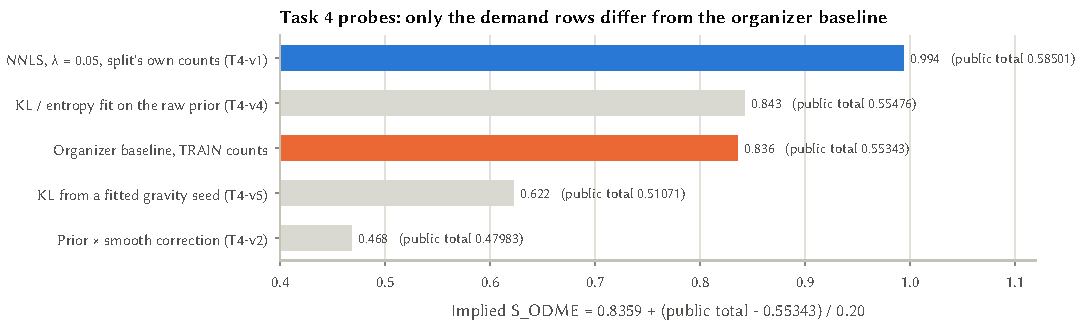
\includegraphics[width=\linewidth]{figures/fig_odme.pdf}
\caption{Implied $\Sodme$ of five demand estimators, each submitted with otherwise identical baseline rows.}\label{fig:odme}
\end{figure}

The organizer's baseline solves the same problem against \emph{training} counts and scores 0.836. Solving it exactly
against the split's own counts and prior scores an implied 0.994. Every attempt to model the prior did worse: an entropy (KL) fit to the raw prior 0.843, a KL fit from
a fitted gravity seed 0.622, and a prior multiplied by a smooth distance correction 0.468. Forensics on the training
split suggested a prior equal to the truth plus positive noise, but no parametric law we fitted, gravity or distance
decay, explained it well enough to help. The whole Task 4 gain came from solving the right system exactly.

\begin{keybox}[Insight]
With a weak prior and a regularizer chosen by the organizers, the scoring reference is itself a regularized solve.
The best estimate is the exact optimum of the same objective on the same split's data; structure that is not in the
objective (gravity, distance decay, entropy) only moved the answer away from the reference. We stopped spending
submissions on Task 4 after the first day.
\end{keybox}

% ============================================================= VALIDATION ==
\section{Analysis of validation results}\label{sec:leaderboard}

\subsection{Exact additive identification}
The three row blocks of a submission are disjoint, and each task is scored only on its own rows. Writing
$B=0.35\,\Sstate+0.15\,\Sphys$ for the block that depends on the state rows,
\begin{equation}
  \Stotal = B + 0.20\,\Sodme + 0.15\,\IoU_{\mathrm{onset}} + 0.15\,\IoU_{\mathrm{ongoing}}
  \label{eq:additive}
\end{equation}
holds exactly. Two submissions that differ in one block therefore measure the change of that block exactly, up to
the five-decimal rounding of reported scores ($\pm5\times10^{-6}$ per score, or about $\pm7\times10^{-5}$ in an IoU).
The organizers' baseline table (\cref{tab:baselines}) anchors absolute values: persistence predicts nothing on onset
windows, so its $\Squeue=0.3017$ is half of an ongoing IoU of 0.6034.

Chaining single-block contrasts from that anchor identifies the values in \cref{tab:components}. The chain is
consistent: rebuilding J1 from its identified parts gives 0.84461, exactly its reported score. Two steps (CT1 and CF1)
changed two blocks at once, so the state and ongoing values after them are bounded rather than identified
(\cref{sec:queue-results}). The split of $B$ between $\Sstate$ and $\Sphys$ is not identifiable.

\begin{table}[h]
\centering\small
\caption{Component values identified from validation scores through \cref{eq:additive}. Generated from the submission
record by \code{docs/scripts/make\_figures.py}.}\label{tab:components}
\begin{tabular}{@{}l l r l@{}}
\toprule
Task & Quantity & Value & Identified from \\
\midrule
Demand & $S_{\mathrm{ODME}}$, organizer baseline (TRAIN counts) & 0.8359 & documented \\
 & $S_{\mathrm{ODME}}$, exact NNLS on the split's own counts & 0.9938 & T4-v1 $-$ BASE \\
\addlinespace[2pt]
State & $B$, weekday--slot historical mean (baseline) & 0.2957 & documented \\
 & $B$, time interpolation & 0.4140 & L0 $-$ U2 \\
 & $B$, first residual GBDT (V1) & 0.4226 & P-persq \\
 & $B$, RS1 residual GBDT & 0.4324 & RC2 $-$ RC1 \\
\addlinespace[2pt]
Onset & IoU, persistence (predicts nothing) & $\approx 0$ & by construction \\
 & IoU, first LightGBM, 13 slots incl.\ $T$ (V1) & 0.6393 & V1 $-$ P-noonset \\
 & IoU, legal 12-slot classifier (U1) & 0.6258 & U1 $-$ P-persq \\
 & IoU, train frequency prior (U3) & 0.4497 & U3 $-$ U2 \\
 & IoU, demand-history completion (CS3) & 0.7116 & CS3 $-$ CS2 \\
 & IoU, joint-mask analogue (J1, kept to ES4) & 0.7499 & J1 $-$ U2 \\
\addlinespace[2pt]
Ongoing & IoU, organizer persistence (eligible cells) & 0.6034 & documented \\
 & IoU, first LightGBM, 13 slots incl.\ $T$ (V1) & 0.5922 & P-noonset \\
 & IoU, same, trained on unfiltered windows & 0.6144 & V1-nh $-$ V1 \\
 & IoU, state at slot $T$ (diagnostic only) & 0.7293 & P-slotT $-$ V1 \\
 & IoU, forward-fill of the last legal value (U2) & 0.7381 & U2 $-$ U1 \\
 & IoU, RQ2 analogue decoder (CS1) & 0.7657 & CS1 identity \\
 & IoU, origin analogue (CS2) & 0.7397 & CS2 $-$ CS1 \\
 & $\Delta$IoU, RQ48 quarter-prior decoder & +0.0313 & CF2 $-$ CF1 \\
 & $\Delta$IoU, occupancy classifier RQ59 & -0.0007 & CF3 $-$ CF2 \\
 & $\Delta$IoU, all-month classifier EQ1 & +0.0026 & ES1 $-$ TF3 \\
\bottomrule
\end{tabular}

\end{table}

Three observations follow. The residual state model added 0.127 to $B$ over the historical-mean baseline, more than
any other single change. Onset forecasting moved from zero to 0.750 IoU, worth 0.112 in the composite score. Ongoing
forecasting, which received most of the research effort after the first week, moved from 0.603 to about 0.83, worth
about 0.034.

\subsection{Decomposition of the improvement}
\Cref{tab:steps} decomposes the improvement from the organizer baselines to ES4 into sixteen measured steps. Each
step is the difference between two validation scores; the RS1 and RQ2 steps follow from additivity.

\begin{table}[h]
\centering\small
\caption{Measured steps from the organizer baselines to ES4.}\label{tab:steps}
\begin{tabular}{@{}r l l r r@{}}
\toprule
Step & Change & Rows changed & $\Delta$ score & Cumulative \\
\midrule
0 & Organizer baselines (anchor) & all & & 0.55343 \\\\
1 & Exact split-specific NNLS demand & Demand & +0.03158 & 0.58501 \\
2 & Residual GBDT state reconstruction & State & +0.12691 & 0.71192 \\
3 & Legal onset classifier (U1) & Onset & +0.09387 & 0.80579 \\
4 & Forward-filled ongoing persistence (U2) & Ongoing & +0.02021 & 0.82600 \\
5 & Joint-mask onset analogue (J1) & Onset & +0.01861 & 0.84461 \\
6 & RS1 state model (RC2 $-$ RC1) & State & +0.00974 & 0.85435 \\
7 & RQ2 ongoing analogue decoder (CS1, by additivity) & Ongoing & +0.00414 & 0.85849 \\
8 & S5 speed correction and Q19 features (CT1) & State, ongoing & +0.00039 & 0.85888 \\
9 & S10 factor flow and S12 covariance speed (CT2) & State & +0.00151 & 0.86039 \\
10 & FS1 gate and Q46 first-crossing classifier (CF1) & State, ongoing & +0.00449 & 0.86488 \\
11 & RQ48 quarter-prior decoder (CF2) & Ongoing & +0.00469 & 0.86957 \\
12 & Three-member sample ensemble (TF3) & State & +0.00034 & 0.86991 \\
13 & All-month ongoing classifier (ES1) & Ongoing & +0.00039 & 0.87030 \\
14 & Gap-1 speed recentering (ES2) & State & +0.00039 & 0.87069 \\
15 & Gap-2 speed recentering (ES3) & State & +0.00044 & 0.87113 \\
16 & Gap 3--6 speed recentering (ES4) & State & +0.00074 & 0.87187 \\
\bottomrule
\end{tabular}

\end{table}

\subsection{Transfer of local proxies}\label{sec:transfer}
Seventeen submissions changed the rows of exactly one task relative to an earlier file (\cref{fig:transfer}). Each was
evaluated because a local proxy or a measured rationale favoured it. The contrast between the two panels of the figure
is the most useful methodological result of this work.

\begin{figure}[htbp]
\centering
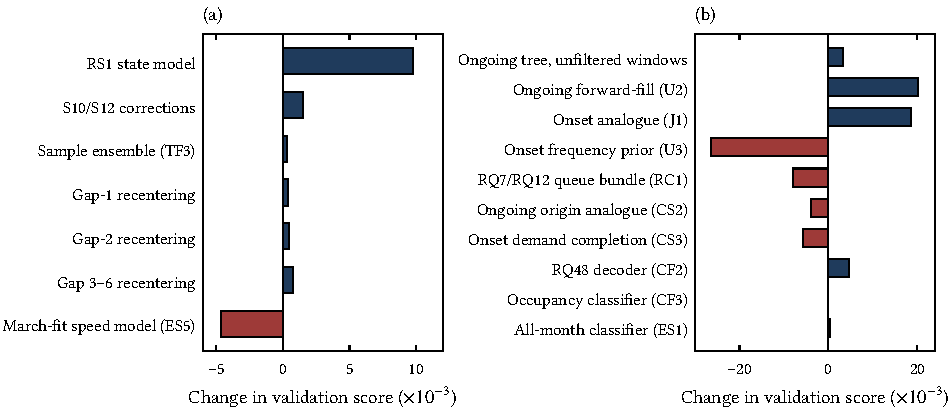
\includegraphics[width=\linewidth]{figures/fig_transfer.pdf}
\caption{Change in validation score of every single-task change: (a) state-only changes, (b) queue-only changes.}\label{fig:transfer}
\end{figure}

\begin{itemize}
  \item \textbf{State changes transferred.} All six state changes selected on held-out training months improved the
        validation score, though by less than the held-out proxies suggested (\cref{sec:state-error}). The single state
        loss, ES5 ($-0.00462$), is the only model fitted and selected on visible cells of the evaluation month itself.
        It lowered visible-cell speed RMSE from 2.545 to 2.006 km/h on every corridor, yet the visible cells were not a
        stand-in for the masked holes.
  \item \textbf{Queue changes did not.} Five of ten queue-only changes lowered the score. CF3's occupancy classifier
        gained 0.0074 to 0.0085 ongoing IoU on visible March proxies and lost 0.0007 on validation; the onset frequency
        prior kept its skill leave-one-month-out on training windows and lost 0.176 onset IoU on validation.
\end{itemize}

Two facts explain the asymmetry. State scores average over millions of cells, so a real improvement is visible; queue
scores average over 80 windows per split. Moreover, the visible-cell and published-window proxies differ in kind from
the hidden targets: visible pseudo-events are noisy observations rather than latent labels, and the published windows
are 80 events from ten days in June.

\subsection{Sampling noise and the private month}
The organizers estimate that queue-window sampling alone moves $\Stotal$ by about 0.0126 (one standard deviation).
The private month has seven incidents against five in the validation month, at different places and times.
Differences of a few thousandths between files are therefore not a reliable forecast of the private ordering, and the
state reconstruction is the most stable part of any composite score.

\subsection{Choice of the final submissions}
Two submissions are scored on the private month. They were chosen for complementary reasons.
\begin{itemize}
  \item \textbf{TF3} is the most defensible artefact: every component was selected on held-out training months under
        pre-registered tests, and the whole file regenerates from the raw release with one command (\cref{sec:repro}).
  \item \textbf{ES4} adds the two later changes that improved the validation score, the all-month ongoing classifier
        and the label-free short-gap recentering, and shares TF3's onset, flow and demand rows exactly.
\end{itemize}
ES5, the only later file, was not selected: it lowered the validation score, and its model was fitted on the
evaluation month.

% ============================================================== NEGATIVE ==
\section{Negative results}\label{sec:negative}

Most of what we built did not ship. We list the rejected branches because they bound what the data support, and
because several are natural first ideas for this benchmark. Each was registered with a fixed gate before its result
was seen; no failed branch was rescued by changing the gate afterwards. Numbers marked \proxy{} are local proxies;
the others are Kaggle public changes. The physics-based reconstructions are in \cref{tab:physics}.

\needspace{14\baselineskip}
{\small
\setlength{\tabcolsep}{4pt}
\begin{longtable}{@{}p{0.11\linewidth} p{0.33\linewidth} p{0.39\linewidth} p{0.11\linewidth}@{}}
\caption{Rejected branches.}\label{tab:negative}\\
\toprule
ID & Idea & Evidence & Decision \\
\midrule
\endfirsthead
\toprule
ID & Idea & Evidence & Decision \\
\midrule
\endhead
\midrule\multicolumn{4}{r}{\footnotesize continued on the next page}\\
\endfoot
\bottomrule
\endlastfoot
\multicolumn{4}{@{}l}{\textbf{\sffamily State}}\\
L0 & Plain time interpolation instead of the residual model & public $-$0.00867 & keep model \\
ES5 & Speed model fitted on odd March days, applied to hidden March holes & visible RMSE 2.545 $\to$ 2.006\proxy{} on every corridor; public $-$0.00462 & rejected \\
--- & Weekday profile from the split's own masked observations & February piece 0.375 vs interpolation 0.790\proxy{} & rejected \\
TS1 & Covariance adaptation of the state model & lost on all ten panels, both development months\proxy & rejected \\
TS2 & Group-RMSE training loss & joint +0.00007\proxy{} but $\Sstate$ fell in both months & failed gate \\
TA2 & Regional spatial modes & lost on all ten panels, both months\proxy & rejected \\
S13 & Density correction allocated by LWR edge coverage & February improved 5 of 10 panels (8 required)\proxy & failed gate \\
FS1 arms & Full flow replacement; replacement only under R3; rank-24 and flow-only wider gates & lost or did not win development\proxy & not used \\
--- & Replace short-gap speeds by the interpolant & ES1 differs from the interpolant by 1.39 km/h (mean absolute) on March one-slot cells, while the interpolant's February RMSE on such cells is 2.37 km/h\proxy & rejected \\
--- & Restore pre-recentering speeds on hard holes (ES6) & undoes the bias shift without restoring model skill & built, withheld \\
--- & Link-by-hour bias split & RMSE 2.7560 $\to$ 2.7567\proxy{} (gate $-$0.15) & failed gate \\
--- & December speed/flow bin calibration & January RMSE 1.6491 $\to$ 1.6450\proxy{} (gate $-$0.05) & failed gate \\
--- & Weekday/weekend split of the link bias & 1.6450 $\to$ 1.6455\proxy & failed gate \\
--- & One-sided and long-gap shells & signal 732 vs bar 850,000 (cell-weighted km$^2$/h$^2$)\proxy & too small \\
--- & Flow recentering on one-slot cells & March link offset 10.9 veh/h RMS (bar 20)\proxy & too small \\
ES0 & Structured inner masks for self-supervision & target and visible-cell gap geometry already identical; structured masks worsened the match\proxy & closed \\
\addlinespace[3pt]
\multicolumn{4}{@{}l}{\textbf{\sffamily Onset}}\\
U3 & Training frequency prior at $T{+}30$ (top three links) & leave-one-month-out 0.558\proxy; public onset IoU 0.626 $\to$ 0.450 & rejected \\
CS3 & Complete onset demand history from TRAIN ramp profiles & public onset IoU 0.750 $\to$ 0.712 & rejected \\
RQ54 & Direct onset action-value regression & training gain, April loss\proxy & rejected \\
RQ60 & Whitened correlation for onset retrieval & lost April and held TRAIN\proxy & rejected \\
--- & Bottleneck placement (highest flow/capacity, largest occupancy rise) & IoU 0 on all 40 published onsets\proxy{} vs analogue 0.936 & rejected \\
--- & Same-month (earlier-day) onset priors & 0.105 and 0.333 vs analogue 0.776 and 0.726\proxy & rejected \\
--- & More or fewer onset neighbours, frozen on odd dates & 50 neighbours 0.706 vs deployed 0.704 on even dates\proxy & no gain \\
--- & Reranker over onset actions & 0.691 vs 0.704\proxy{} on even dates & rejected \\
\addlinespace[3pt]
\multicolumn{4}{@{}l}{\textbf{\sffamily Ongoing}}\\
RC1 & RQ7 ongoing with RQ12 onset bundle & public $-$0.00798 vs J1 queues & rejected \\
CS2 & Five-minute analogue origins & public $-$0.0039 & rejected \\
CF3 & Occupancy-aware classifier RQ59 & +0.0074 to +0.0085\proxy{} on March; public $-$0.0001 & selected, lost \\
Q22 & Neural blend with the Q19 classifier & failed its confirmation gate\proxy & rejected \\
Q34 & Better masked-history imputation & history RMSE 0.055 $\to$ 0.026\proxy, forecast lost on both samples & rejected \\
Q36 & Explicit site identifiers & failed confirmation\proxy & rejected \\
TQ1, TQ2 & Event-census queue models & TQ2 February +0.0038, published June $-$0.0010\proxy & failed gate \\
FQ2, FQ3 & Exact Bernoulli first-crossing law; three-model blend & April confirmation losses\proxy & rejected \\
RQ49--52 & Copula ranks; phase experts; space--time binary field; hindcaster & March or April losses, or no future-overlap gain\proxy & rejected \\
RQ53P & Partial likelihood over 64 trajectories per link & March +0.0042, April +0.0013\proxy{} (bar 0.003) & failed gate \\
RQ55 & Better optimization of the RQ48 utility & higher objective, lower overlap in both months\proxy & rejected \\
RQ56--58 & Per-horizon classifiers; auxiliary thresholds; date-cluster bagging & below the 0.003 bar or losses\proxy & rejected \\
RQ61--62 & Scaling (similarity) augmentation of the traffic law & lost confirmation, or lost to RQ59\proxy & rejected \\
--- & Front rollout from the legal hour & 0.234 vs persistence 0.755\proxy & rejected \\
--- & Median remaining-duration rollout & 0.263 vs forward-fill 0.665\proxy & rejected \\
--- & Yesterday's masked queue; clock-time prior & 0.249 vs 0.569; 0.538 vs 0.718\proxy & rejected \\
--- & History-only queue-dynamics model & 0.831 vs analogue 0.836 (bar 0.856)\proxy & failed gate \\
--- & Rerankers, per-link copies, neighbour-bit model & see \cref{sec:queue-results} & failed gates \\
--- & Same-month March library; March-fit binary model & 0.324 and 0.794 vs 0.836\proxy{} on even dates & rejected \\
--- & Newell envelope rolled six steps & ongoing 0.162 vs 0.866; onset 0.006 vs 0.675\proxy & rejected \\
\addlinespace[3pt]
\multicolumn{4}{@{}l}{\textbf{\sffamily Demand}}\\
T4-v2, v4, v5 & Smooth correction, entropy fit, gravity seed & implied $\Sodme$ 0.468, 0.843, 0.622 vs 0.994 & rejected \\
\end{longtable}}

\begin{notebox}[What the failures have in common]
Three patterns recur. Models fitted to the evaluation month's visible cells (ES5, same-month profiles, the March
library) learned that month's visible behaviour and did not transfer to its hidden cells. Physically motivated
dynamics (rollouts, envelopes, solvers) lost to empirical analogues and to temporal evidence, because the forcing
that matters, incidents and the moment of breakdown, is not in the twelve legal slots. And better local objectives
(RQ55's utility, Q34's imputation) did not imply better forecasts: improvements must be measured on the score that
counts, on held-out data.
\end{notebox}

% ============================================================ DISCUSSION ==
\section{Discussion}\label{sec:discussion}

\subsection{What the benchmark taught us about traffic}
\begin{enumerate}
  \item \textbf{At five-minute resolution, time beats space.} Links are short (many are a few hundred metres) and masked
        holes span one to five links. A wave crosses a link in seconds, so a link's own readings five minutes before and
        after carry more information about a hole than its neighbours at the same moment (\cref{sec:physics,sec:state-error}).
  \item \textbf{Missing is not free flow.} About a quarter of last readings are missing or ineligible. Treating a dropped
        sensor as ``not queued'' cost 0.135 ongoing IoU; the forecaster must carry the last observed state forward.
  \item \textbf{Onsets are recurrent in location and random in extent.} The head of a new queue is usually a known
        bottleneck, but how far it extends by $T{+}30$ depends on when breakdown happens inside the last five minutes,
        which the legal hour cannot show.
  \item \textbf{Queues have memory beyond the hour.} Clearing queues in the training windows are old (300--780 minutes)
        and small; most growing ones are 10--20 minutes old. Queue age is visible only before $T{-}60$, outside the
        contract we kept.
  \item \textbf{A new month brings a link-level offset.} A model trained on other months carries per-link means into the
        new month that the month's own anchors contradict. A label-free recentering on short gaps removed part of it.
  \item \textbf{With a weak prior, demand is an optimization problem, not a modelling one.} The exact regularized solve on the
        split's own counts reached an implied 0.994.
\end{enumerate}

\subsection{Where the remaining score is}
\Cref{tab:budget} combines the identified components with the organizers' perfect-answer scores. The state block
$B$ is bounded rather than identified after CT1 and CF1; the ongoing value inherits that bound.

\begin{table}[h]
\centering\small
\caption{Error budget of ES4 on the validation month, in units of the composite score. ``Room'' is the ceiling minus
our contribution; the value of $B$ is bounded rather than identified.}\label{tab:budget}
\begin{tabular}{@{}l r r r r@{}}
\toprule
Block & Component value & Contribution & Ceiling & Room \\
\midrule
Demand, $0.20\,\Sodme$ & 0.9938 & 0.1988 & 0.2000 & 0.0012 \\
Onset, $0.15\,\IoU$ & 0.750 & 0.1125 & 0.1500 & 0.0375 \\
Ongoing, $0.15\,\IoU$ & 0.827--0.832 & 0.124--0.125 & 0.1500 & 0.025--0.026 \\
State and physics, $B$ & & 0.4358--0.4366 & 0.4945 & 0.058 \\
\midrule
Total & & 0.87187 & 0.9945 & 0.1226 \\
\bottomrule
\end{tabular}
\end{table}

The budget also bounds what further queue work can achieve. With our state and demand blocks unchanged, a perfect
queue forecast ($\Squeue=1$) would reach a composite score of about 0.935. Larger improvements therefore require a
better state-and-physics block, most plausibly in conservation, where the block has 0.058 of room and our local
instruments are weakest.

\subsection{Limitations}
\begin{itemize}
  \item No private score was available for either file at the time of writing, and the validation difference between
        them (0.00196) is far below the queue-sampling standard deviation.
  \item Local proxies were reused across many studies; March and April visible events in particular were examined
        repeatedly, and their confidence intervals do not correct for that reuse.
  \item The three ensemble members share features and overlapping samples. Averaging reduces sampling variance, not
        bias they share.
  \item The gap recentering is a link mean, not a model of shocks; gaps of eight or more slots, which failed the bias
        test, keep the uncorrected field.
  \item The queue selection problem is open: the candidate set contains much better masks than the ones chosen.
  \item Our Task 2 contract is stricter than the rules. It excludes slot $T$ and same-day data before $T{-}60$, which the
        rules allow, and so leaves the queue-age signal unused.
  \item The local physics proxy uses observed accumulation in place of the withheld boundary flux and is not the
        official physics score.
  \item ES4 regenerates from the release only up to its parent: the all-month classifier weights behind ES1 are not in
        this repository (\cref{sec:repro}).
\end{itemize}

\subsection{Future work}
\begin{itemize}
  \item \textbf{Learn the choice among whole masks.} Train a ranker on first-crossing windows whose target is each
        candidate's realized IoU, and decide by expected IoU over structured outcomes rather than a fixed mixture
        \cite{nowozin2014}. The 0.10 gap between the chosen and the best candidate is the largest identifiable lever.
  \item \textbf{Model onset extent as breakdown timing.} Treat the extent at $T{+}30$ as a function of a breakdown time with
        a hazard learned from the legal hour, instead of copying neighbour extents.
  \item \textbf{Use legal same-day context.} The rules allow data before $T{-}60$. Queue age is a strong predictor of
        clear-versus-grow on training windows and deserves a pre-registered test.
  \item \textbf{Conservation as a soft target inside the learner.} Every hard physics projection lost. A penalty on the
        conservation residual of neighbouring predictions, learned jointly with the residual model, has not been tried.
  \item \textbf{Hierarchical month offsets.} Extend the recentering to flow and to longer gaps with a shrinkage estimator
        that borrows strength across links, instead of a hard 100-cell threshold.
\end{itemize}

% ======================================================= REPRODUCIBILITY ==
\section{Reproducibility}\label{sec:repro}

\subsection{Environment and hardware}
All production runs used CPU only on one AWS EC2 \code{r7i.2xlarge} instance (8 vCPU, 64 GiB RAM, Ubuntu with glibc
2.39) and Python 3.12.3 with the pinned packages in \cref{tab:env}. No GPU is needed. The clean regeneration of TF3
took 1 h 33 min with six threads, including rebuilding every cache from the raw release. Regenerating ES4 is estimated
at about 3 hours or less and both files at about 4.5 hours or less; neither total has been measured as one run. Peak
memory was not recorded, so 64 GiB is what was used and not a proven minimum. The release is 7.76 GiB as a zip file, its
dense caches take 4.1 GiB, and we recommend at least 40 GiB of free disk.

\paragraph{Kaggle Notebook} The method cannot be run inside a Kaggle Notebook as packaged and was never run in one. It
was developed and operated as a chain of command-line stages under an exact pinned environment on a larger machine than
a standard notebook provides. We therefore supply a repository and a written account of how it was run,
\code{REPRODUCIBILITY.md}, which lists the versions, preprocessing steps, seeds, commands and verification status.

\begin{table}[h]
\centering\small
\caption{Pinned inference environment (\code{requirements.txt}) and the licence of each dependency.}\label{tab:env}
\begin{tabular}{@{}l l l@{}}
\toprule
Package & Version & Licence \\
\midrule
NumPy \cite{harris2020} & 2.5.3 & BSD-3-Clause \\
pandas & 3.0.6 & BSD-3-Clause \\
SciPy \cite{virtanen2020} & 1.18.1 & BSD-3-Clause \\
PyArrow & 25.0.1 & Apache-2.0 \\
LightGBM \cite{ke2017} & 4.7.0 & MIT \\
scikit-learn & 1.9.1 & BSD-3-Clause \\
\bottomrule
\end{tabular}
\end{table}

\subsection{Commands}
The repository has one entry point. The competition release is not redistributed; \code{-{}-release-root} is the
directory that contains \code{submission\_key.csv}, \code{corridors/} and \code{task2/}.

\smallskip
\noindent\begin{minipage}{\linewidth}
\small
\begin{verbatim}
# 1. verify the final archives and the TF3 code bundle (standard library only)
python reproduce.py

# 2. regenerate TF3 from the raw release and the saved weights
python -m pip install -r requirements.txt
python reproduce.py --submission tf3 --release-root /path/to/release \
                    --out /path/to/new_tf3 --threads 6

# 3. regenerate ES4 from the raw release, including EQ1 retraining
python reproduce.py --submission es4 --release-root /path/to/release \
                    --out /path/to/new_es4 --threads 6

# 4. regenerate both selected files, sharing one set of caches
python reproduce.py --submission all --release-root /path/to/release \
                    --out /path/to/new_all --threads 6
\end{verbatim}
\end{minipage}

\subsection{What has been verified}
\begin{itemize}
  \item \textbf{TF3, end to end.} The bundled driver rebuilds every cache and prediction component from the release
        and the saved TRAIN weights, then compares all 6,980,503 rows with the submitted file. On the clean run every queue
        label matched exactly and the largest continuous difference was $1.82\times10^{-12}$. This verifies saved-weight
        inference; the refit procedure, seeds and inventories are recorded, but an independent retraining was not run.
  \item \textbf{ES4.} The final archive is in the repository and its checksum is verified by \code{reproduce.py}.
        Row-level comparison confirms that ES4 is TF3 plus 247 ongoing-queue labels and 5,825,667 recentered speeds.
        \code{code/regenerate\_es4.py} runs the original stage scripts from the release through ES1, ES2, ES3 and ES4 and
        compares every row with the frozen file. It has been exercised on synthetic data but \textbf{has not yet been run
        on the real release}. The EQ1 classifier weights existed only on the instance used during the competition, which
        no longer exists, so the command retrains EQ1 from the release; whether that model is identical to the original
        is not yet known. Only the 247 EQ1-dependent labels depend on this. TF3 scored 0.00196 (0.22\,\%) below ES4 on the
        validation month.
\end{itemize}

\subsection{Artefacts and checksums}
\begin{table}[H]
\centering\small
\caption{SHA256 of the main artefacts. The first three are verified by \code{python reproduce.py}.}\label{tab:sha}
\begin{tabular}{@{}l l@{}}
\toprule
Artefact & SHA256 \\
\midrule
\code{submissions/submission\_TF3.zip} & \sha{2ae94d422399c7248297487fc8f45d737de0e024fbad32b6a360c290bbabca7a} \\
\code{submissions/submission\_ES4.zip} & \sha{ce03386b42e33bc6c726b09c0b64b791f294ea3abeb88d7e310552bb080c04bb} \\
\code{vendor/reproduction\_TF3.zip} & \sha{dce93b3f2a38d27014497ec1a563cc1e2d032da11c499234f226c72093678cd7} \\
TS3 frozen rule & \sha{61499049f1cced66927eff4c9e9c99bb611093c33c3a31de98ebd436940883d5} \\
TS3 final model manifest & \sha{8ed505b54215cd88706e95dedc5b4fbee3f435e228560f8d71d018b546cf6acb} \\
TS3 registered protocol & \sha{fcc9f299f32bc0df8dc68749df21ceb1d2bc2609fc3d2a21b15a85913c84aec0} \\
Q46 ongoing classifier (TF3) & \sha{2816e1d3f3c233416327591c6659cd9e80a25f0054431f1b1d4ee23735b2ab46} \\
EQ1 ongoing classifier, 800 trees (ES4) & \sha{cb626813e621064594f6956344df81d7d8879e65ebc23ae2f164a2f8f6f9ac9f} \\
\bottomrule
\end{tabular}
\end{table}

\subsection{Seeds and data membership}
TS3 members draw their training rows with \code{random\_state} equal to the member seed (20261104 or 20261204) plus
the panel index; the RS1 models use LightGBM seed 20261001 and samples drawn with 20261001 plus the panel index; Q46's
training windows use 20261046 plus the panel index; EQ1's additional windows use 20261240 plus the panel index; both
classifiers use LightGBM seed 20261002. At inference, the only seed is the S10 randomized start, $20261003 + 100\times$
panel index $+$ month. The fit manifests in the TF3 bundle record the fitting months, row counts and input
hashes of every saved model, and two independent audits recomputed every stored weekday profile (31,783,763 fitting
rows) exactly.

\subsection{External data and licence declaration}
No external dataset, pretrained model, paid or rate-limited API or proprietary dependency was used. The only data are
the competition release, used under the competition rules and not redistributed here. All software dependencies are
open source under the licences in \cref{tab:env}. Figures were produced with Matplotlib and the report with \LaTeX.
Our own code is released under the MIT licence.

% ============================================================ CONCLUSION ==
\section{Conclusion}\label{sec:conclusion}

We built a pipeline for TrafficFlowBench through measured, single changes and kept a strict information boundary
throughout. Its strongest parts are simple: learn the residual of temporal interpolation, choose whole onset masks
by expected IoU, carry dropped sensors forward, and solve the demand system exactly. Its weakest part is equally
clear: the choice among good candidate queue futures. Using the additivity of the composite score, we treated our
evaluated submissions as a controlled ablation. It showed that state improvements selected on held-out months transfer
to a new month, whereas queue proxies often do not. We hope that the negative results, in particular that four kinds
of physics-based reconstruction lost to temporal evidence on held-out months, will be useful to future work on this
benchmark.

Both final submissions are documented and checksummed, and the reconstruction submission TF3 regenerates from the raw
release with a single command.


\bibliographystyle{unsrtnat}
{\small\bibliography{references}}

\appendix
% ============================================================== APPENDIX ==
\needspace{20\baselineskip}
\section{Complete submission history}\label{app:history}

\begin{table}[H]
\centering\footnotesize
\caption{All 31 Kaggle submissions of the team, in order. Public scores are Kaggle results; the two selected files
are in bold. Generated from \code{docs/data/submissions.csv}.}\label{tab:history}
\setlength{\tabcolsep}{4.5pt}
\begin{tabular}{@{}r l l r@{}}
\toprule
\# & ID & Content & Validation score \\
\midrule
1 & BASE & Organizer baselines for all tasks & 0.55343 \\
2 & T4-v2 & ODME: prior $\times$ smooth correction & 0.47983 \\
3 & T4-v4 & ODME: KL/entropy fit to the prior & 0.55476 \\
4 & T4-v5 & ODME: KL from a gravity seed & 0.51071 \\
5 & T4-v1 & ODME: exact NNLS on the split's own data & 0.58501 \\
6 & V1 & First GBDT state, LightGBM queues & 0.80613 \\
7 & P-persq & V1 state with persistence queues & 0.71192 \\
8 & P-noonset & V1 with onset rows set to zero & 0.71024 \\
9 & V1-nh & V1, ongoing tree on unfiltered windows & 0.80946 \\
10 & P-slotT & Ongoing set from slot $T$ (diagnostic) & 0.82669 \\
11 & U1 & Legal onset classifier (12 slots) & 0.80579 \\
12 & U2 & U1 with forward-filled ongoing persistence & 0.82600 \\
13 & J1 & U2 with the joint-mask onset analogue & 0.84461 \\
14 & L0 & U2 with time-interpolated state & 0.81733 \\
15 & U3 & U2 with an onset frequency prior & 0.79958 \\
16 & RC1 & RQ7 ongoing and RQ12 onset & 0.83663 \\
17 & RC2 & RC1 with RS1 state & 0.84637 \\
18 & CS1 & RS1 state, RQ2 ongoing, J1 onset & 0.85849 \\
19 & CS2 & CS1 with origin-analogue ongoing & 0.85459 \\
20 & CS3 & CS2 with onset demand completion & 0.84885 \\
21 & CT1 & S5 speed correction, Q19 ongoing & 0.85888 \\
22 & CT2 & CT1 with S10/S12 state & 0.86039 \\
23 & CF1 & FS1 gate, Q46 ongoing & 0.86488 \\
24 & CF2 & CF1 with RQ48 decoder & 0.86957 \\
25 & CF3 & CF2 with occupancy classifier & 0.86947 \\
26 & \textbf{TF3} & CF2 with three-member ensemble & \textbf{0.86991} \\
27 & ES1 & TF3 with all-month ongoing classifier & 0.87030 \\
28 & ES2 & ES1 with gap-1 recentering & 0.87069 \\
29 & ES3 & ES2 with gap-2 recentering & 0.87113 \\
30 & \textbf{ES4} & ES3 with gap 3--6 recentering & \textbf{0.87187} \\
31 & ES5 & ES4 with March-fit speed model & 0.86725 \\
\bottomrule
\end{tabular}

\end{table}

\needspace{12\baselineskip}
\section{Glossary of identifiers}\label{app:glossary}

{\small
\begin{longtable}{@{}p{0.13\linewidth} p{0.83\linewidth}@{}}
\toprule
ID & Meaning \\
\midrule
\endfirsthead
\toprule
ID & Meaning \\
\midrule
\endhead
\bottomrule
\endlastfoot
BASE & The organizer's baselines for all four tasks, submitted as an anchor (0.55343). \\
T4-v$n$ & Task 4 probes: only demand rows differ from BASE. v1 is the exact split-specific NNLS that every later file uses. \\
V1 & First full file: residual GBDT state, LightGBM queues reading 13 slots including $T$. Superseded. \\
P-$\ast$ & Probes that isolate one component: P-persq (persistence queues), P-noonset (onset zeroed), P-slotT (diagnostic, reads slot $T$). \\
U1, U2, U3 & First files under the twelve-slot contract: legal onset classifier; plus forward-filled ongoing persistence; plus an onset frequency prior. \\
J1 & U2 with the joint-mask onset analogue. Its onset and demand rows are retained in both selected files. \\
L0 & U2 with time-interpolated state; an ablation of the residual model. \\
RS1 & Enhanced residual state model (92 features, density reconciliation), refit on all nine TRAIN months. \\
RQ$n$, Q$n$ & Queue research arms. RQ2: trajectory-analogue decoder. Q19: local and distance-scaled ongoing features. Q46: first-crossing classifier. RQ48: quarter-weight decoder utility. RQ59: occupancy classifier. \\
RC$n$, CS$n$ & 2 October candidates combining RS1 state with queue variants. \\
S5, S10, S12 & Free-branch corrections: rank-8 covariance speed; rank-12 temporal factor flow; spatial-covariance conditional speed. \\
FS1 & The widened, half-strength free-branch gate combining S10 and S12. \\
CT$n$, CF$n$ & 3 October candidates. CT1: S5 + Q19. CT2: + S10/S12. CF1: + FS1 + Q46. CF2: + RQ48. CF3: + RQ59 (lost). \\
TS3 / TF3 & Three-member fixed sample ensemble of the state model / the submission that carries it. Selected. \\
EQ1 & Ongoing classifier refit on first crossings from all nine TRAIN months, 800 trees. \\
ES1--ES5 & TF3 + EQ1 (ES1); + gap-1, gap-2 and gap 3--6 recentering (ES2--ES4, ES4 selected); + March-fit speed model (ES5, lost). \\
Shell & Target cells whose farther temporal anchor lies a given number of five-minute slots away. \\
Proxy & Any locally computed score; never a leaderboard number. \\
\end{longtable}}

\end{document}
